\documentclass[10pt,twocolumn]{article}
\usepackage[a4paper,margin=0.85in]{geometry}
\setlength{\columnsep}{0.28in}
\raggedbottom

\usepackage[T1]{fontenc}
\usepackage[utf8]{inputenc}
\usepackage{lmodern}
\usepackage{amsmath,amssymb}
\usepackage{booktabs}
\usepackage{array}
\usepackage{graphicx}
\usepackage{tikz}
\usetikzlibrary{arrows.meta,positioning,fit,backgrounds,calc}
\usepackage{hyperref}
\hypersetup{
  colorlinks=true,
  linkcolor=black,
  citecolor=black,
  urlcolor=blue,
  pdftitle={ReproBot -- Final Project Report},
  pdfauthor={Aleyna Kutuk, Engincan Varan, Gul Korkut, Goktug Mert Ozdogan}
}
\usepackage{xcolor}
\usepackage{caption}
\usepackage{pifont}

\definecolor{builtc}{HTML}{1B6F50}
\definecolor{missingc}{HTML}{97303F}
\definecolor{loopc}{HTML}{0E6E78}
\definecolor{warnc}{HTML}{97590C}

\newcommand{\built}{\textcolor{builtc}{\ding{51}}}
\newcommand{\absent}{\textcolor{missingc}{\ding{55}}}
\newcommand{\partl}{\textcolor{warnc}{$\sim$}}
\newcolumntype{L}[1]{>{\raggedright\arraybackslash}p{#1}}
% Wide tables need every point of the text block; 4pt inter-column padding still
% reads cleanly with booktabs rules and keeps them inside the margin.
\newcommand{\squeeze}{\setlength{\tabcolsep}{4pt}}

\renewcommand{\topfraction}{0.9}
\renewcommand{\dbltopfraction}{0.9}
\renewcommand{\bottomfraction}{0.8}
\renewcommand{\textfraction}{0.07}
\renewcommand{\floatpagefraction}{0.75}
\renewcommand{\dblfloatpagefraction}{0.75}
\setcounter{topnumber}{3}
\setcounter{dbltopnumber}{3}
\setcounter{totalnumber}{5}

\title{\textbf{ReproBot: A Multi-Agent System for Automated Scientific Paper Replication}\\[0.4em]
\large Final Project Report}
\author{
  Aleyna Kütük \\ \small\texttt{aleynakutuk10@gmail.com}
  \and
  Engincan Varan \\ \small\texttt{engincanvaran@gmail.com}
  \and
  Gül Korkut \\ \small\texttt{serifegulkorkut@gmail.com}
  \and
  Göktuğ Mert Özdoğan \\ \small\texttt{goekmeroz@gmail.com}
}
\date{inzva AI Projects \#10 \\ 10.10.2026}


\begin{document}
\maketitle

\begin{abstract}
ReproBot reads a machine learning paper's PDF and returns a replication report. It transcribes
the paper with a vision-language model, extracts its claims and experimental setup into
structured fields, generates a self-contained training script, executes that script in a Docker
sandbox while watching the learning curve for signs that training is not healthy, judges the
reproduced number against the paper's claim with explicit arithmetic, reviews the generated code
against the paper, and renders the result as Markdown. Failures at either end --- a script that
crashes and a number that misses --- are fed back to the code generator through one bounded
retry loop. This report presents the finished system and everything it has measured. Five papers
spanning five model families were reproduced at their own full settings and all five passed,
two of them beating the paper's own number. Three of those papers were then carried from PDF to
report three times each: 9 of 9 runs reproduced their claim, and every run reached the full stage
on its first attempt. The central finding is about where the remaining disagreement comes from:
every difference between runs of the same paper traced to exactly one detail that paper never
states, and we could name it each time --- a fully specified protocol gave three independently
generated scripts bit-identical values, while an unstated cross-validation shuffle and an
unstated data split each moved the result in a way we can explain. A loop-on/loop-off ablation
shows the retry loop changed 1 of 5 verdicts, and that the system's real defence against
publishing a wrong number is not the retries but the guards: a live check-up that halts an
unhealthy run, and a Critic that refuses to rule on one. We make no fidelity claim for the
eight-paper CIFAR-10 set: a full \emph{Wide Residual Networks} run measures at about 22 days on
the project's CPU, and a one-epoch run proves that a script executes, never that its number is
right.
\end{abstract}

\section{Introduction}
\label{sec:intro}

Most published machine learning results are reproducible in principle and expensive to reproduce
in practice. The method is in the prose, the numbers are in the tables, and the thousand small
decisions in between --- which split, which initialisation, which library version's defaults ---
are in neither. ReproBot automates the whole path: paper in, replication report out, with every
guess it had to make written down.

The system is a pipeline of seven stages and two bounded retry loops, coordinated through one
shared-memory state object. It is complete: every stage in the project plan exists, has run on
real papers, and is verified by execution rather than by inspection. This report is
self-contained --- it assumes no earlier reading --- and leads with results, because the
results are the point.

Its contributions are:

\begin{itemize}
  \item \textbf{Five full-fidelity replications across five model families}, each judged by
    arithmetic rather than by eye, with two reproductions better than the paper's own number
    (Section~\ref{sec:results}).
  \item \textbf{A repeatability measurement}: three papers carried from PDF to report three
    times each, 9 of 9 passing (Section~\ref{sec:repeat}).
  \item \textbf{The report's main finding}: run-to-run variance is a property of the paper, not
    a defect of the system, and in every case we could name the single unstated detail
    responsible (Section~\ref{sec:unstated}).
  \item \textbf{An explicit, model-proof verdict}: the tolerance is arithmetic over the claim's
    own precision and the run's own measured spread, and no model can change it
    (Section~\ref{sec:verdict}).
  \item \textbf{The project plan's headline ablation}, loop on against loop off, reported
    honestly including where the loop bought nothing (Section~\ref{sec:experiments}).
  \item \textbf{Two documented paper sets}, one CPU-sized and one GPU-bound, and a plain
    statement of which results exist for which (Section~\ref{sec:sets}).
\end{itemize}

\section{The System}
\label{sec:system}


\begin{figure*}[tbp]
\centering
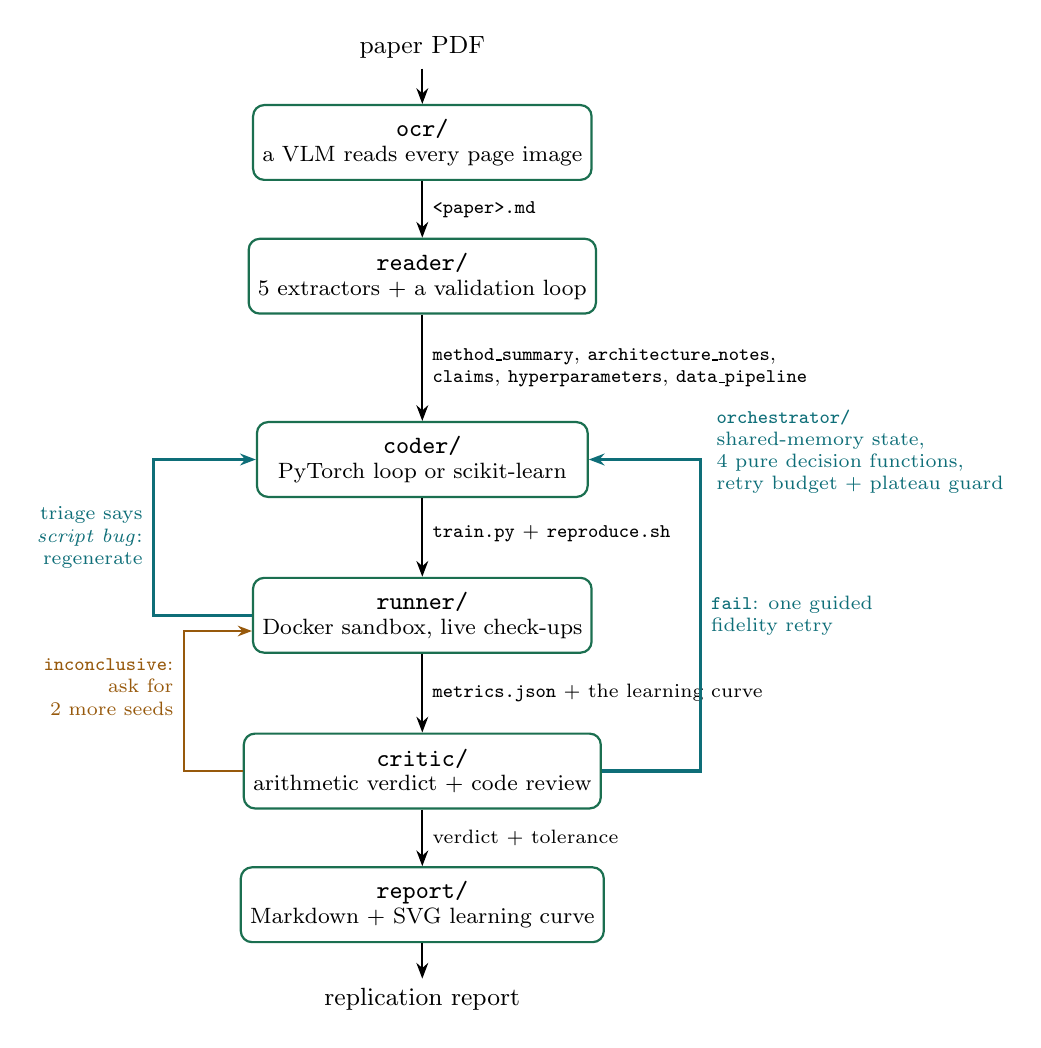
\begin{tikzpicture}[
  node distance=0.72cm and 1.5cm,
  stage/.style={draw, rounded corners, minimum width=4.2cm, minimum height=0.95cm,
    align=center, font=\small, thick, draw=builtc},
  arr/.style={-{Stealth[length=2mm]}, thick},
  looparr/.style={-{Stealth[length=2mm]}, very thick, draw=loopc},
  guardarr/.style={-{Stealth[length=1.8mm]}, thick, draw=warnc},
  lbl/.style={font=\scriptsize, align=left},
  looplbl/.style={font=\scriptsize, align=left, text=loopc}
]
  \node[font=\small, align=center] (pdf) {paper PDF};
  \node[stage, below=0.45cm of pdf] (ocr) {\texttt{ocr/}\\[-2pt]\footnotesize a VLM reads every page image};
  \node[stage, below=of ocr] (reader) {\texttt{reader/}\\[-2pt]\footnotesize 5 extractors + a validation loop};
  \node[stage, below=1.35cm of reader] (coder) {\texttt{coder/}\\[-2pt]\footnotesize PyTorch loop or scikit-learn};
  \node[stage, below=1.0cm of coder] (runner) {\texttt{runner/}\\[-2pt]\footnotesize Docker sandbox, live check-ups};
  \node[stage, below=1.0cm of runner] (critic) {\texttt{critic/}\\[-2pt]\footnotesize arithmetic verdict + code review};
  \node[stage, below=of critic] (report) {\texttt{report/}\\[-2pt]\footnotesize Markdown + SVG learning curve};
  \node[font=\small, align=center, below=0.45cm of report] (out) {replication report};

  \draw[arr] (pdf) -- (ocr);
  \draw[arr] (ocr) -- node[right, lbl] {\texttt{<paper>.md}} (reader);
  \draw[arr] (reader) -- node[right, lbl]
    {\texttt{method\_summary}, \texttt{architecture\_notes},\\
     \texttt{claims}, \texttt{hyperparameters}, \texttt{data\_pipeline}} (coder);
  \draw[arr] (coder) -- node[right, lbl, pos=0.45] {\texttt{train.py} + \texttt{reproduce.sh}} (runner);
  \draw[arr] (runner) -- node[right, lbl] {\texttt{metrics.json} + the learning curve} (critic);
  \draw[arr] (critic) -- node[right, lbl] {verdict + tolerance} (report);
  \draw[arr] (report) -- (out);

  % the two feedback edges, both bounded
  \draw[looparr] (runner.west) -- ++(-1.25,0) |- node[pos=0.25, left, looplbl, align=right]
    {triage says\\ \emph{script bug}:\\ regenerate} (coder.west);
  \draw[looparr] (critic.east) -- ++(1.25,0) |- node[pos=0.25, right, looplbl, align=left]
    {\texttt{fail}: one guided\\ fidelity retry} (coder.east);
  \draw[guardarr] (critic.west) -- ++(-0.75,0) |- node[pos=0.3, left, font=\scriptsize, text=warnc, align=right]
    {\texttt{inconclusive}:\\ ask for\\ 2 more seeds} ([yshift=-0.2cm]runner.west);

  \node[looplbl, anchor=west] at ([xshift=1.5cm, yshift=0.1cm]coder.east)
    {\textbf{\texttt{orchestrator/}}\\ shared-memory state,\\ 4 pure decision functions,\\
     retry budget + plateau guard};
\end{tikzpicture}
\caption{ReproBot, complete. Every stage is built and verified by execution. Two feedback edges
close the loop: the Runner's triage routes a script bug back to the Coder, and the Critic routes a
fidelity failure back as one guided retry, or asks the Runner for extra seeds instead of ruling.
Both are bounded by the Orchestrator's budgets and by a plateau guard that stops a retry which is
not changing the script.}
\label{fig:pipeline}
\end{figure*}


Figure~\ref{fig:pipeline} shows the whole system; Table~\ref{tab:stages} says what each stage
does, what it spends a model call on, and what it checks without one. The design rule throughout
is that anything decidable by arithmetic is decided by arithmetic: a model is called where
judgement is genuinely needed --- reading a figure, writing code, diagnosing a traceback,
reviewing an implementation --- and nowhere else.

\begin{table*}[tbp]
\centering
\small
\caption{The seven stages. Each is a top-level folder with the same command-line shape
(\texttt{-{}-input}, \texttt{-{}-output}, skip what is already done), so any stage can be run
alone or as part of the loop.}
\label{tab:stages}
\squeeze
\begin{tabular}{L{0.16\textwidth}L{0.28\textwidth}L{0.21\textwidth}L{0.25\textwidth}}
\toprule
Stage & What it does & Model calls & Checked without a model \\
\midrule
\texttt{ocr/} & Renders every PDF page to an image and transcribes it, reading figures as well
  as text & One per page & --- \\
\texttt{reader/} & Five structured extractions --- method summary, architecture notes, claims,
  hyperparameters, data pipeline --- then a validation pass that re-runs only the stage a flag
  belongs to & Six, all forced structured output & Bounded at three validation passes;
  truncation, empty and double-encoded payloads caught centrally \\
\texttt{coder/} & One self-contained training script: a plain PyTorch loop for neural models, a
  scikit-learn estimator for classical ones & One & \texttt{ast.parse}; all nine required
  command-line flags present; the learning-curve progress contract \\
\texttt{runner/} & Runs \texttt{reproduce.sh <mode>} in Docker over four escalating stages,
  stopping at the first failure & One triage call, and only on a genuine non-timeout failure &
  Seven live check-up rules that can kill the container; per-stage timeouts; success and timeout
  decided mechanically \\
\texttt{orchestrator/} & Holds the shared-memory state and drives the retry loop as four pure
  decision functions & None & Plateau guard on regenerated scripts; retry and seed budgets \\
\texttt{critic/} & Judges the reproduced number against the claim, and reviews the code against
  the paper & One review call & The verdict itself: arithmetic only. Every citation in the review
  is checked to exist \\
\texttt{report/} & Renders the state object as Markdown with an SVG learning curve & None & Every
  number copied from the state; the tolerance printed with every verdict \\
\bottomrule
\end{tabular}
\end{table*}

\textbf{The loop.} Two feedback edges close it. On an execution failure, a small model classifies
the failure as a bug in the generated script or a problem with the container; a script bug is
routed back to the Coder as a specific complaint and the script is regenerated. On a fidelity
failure, the Critic's verified findings and the Coder's own list of unstated guesses become the
feedback for one guided retry. Both edges are bounded: a retry budget, a single fidelity retry
per paper, and a plateau guard that compares each regenerated script with its predecessor and
stops early when the ``fix'' is not changing anything.

\textbf{The parts that must not be wrong are tested.} The pure logic --- the Critic's arithmetic,
the loop's four decision functions, the seven check-up rules and the report renderer --- is
covered by 102 replay tests, built from real recorded learning curves rather than synthetic
shapes, including every false positive found end to end.

\textbf{What the stages run on.} The Runner's interface is \texttt{reproduce.sh <mode>} and
nothing else --- it never builds a \texttt{python} command and never passes a flag --- so a paper
whose script needs entirely different arguments changes only its own \texttt{reproduce.sh}. The
four modes escalate: \texttt{probe}, a few optimiser steps; \texttt{smoke}, one epoch on a small
slice; \texttt{capped}, a few epochs on a small slice; and \texttt{full}, the paper's own setup.
The Critic may additionally ask for \texttt{seed2} and \texttt{seed3}, which are \texttt{full}
again with another seed.

\section{Results}
\label{sec:results}

\subsection{Fidelity: five papers, five model families}

Table~\ref{tab:fidelity} is the headline result. Five papers were reproduced at their own full
settings --- not a reduced proxy --- and judged by the arithmetic of
Section~\ref{sec:verdict}. All five passed. Two reproductions are better than the paper's own
number by more than the tolerance band, which the Critic records as \texttt{exceeds\_claim}.
Figure~\ref{fig:curves} shows four of the implementations learning.

\begin{table*}[tbp]
\centering
\small
\caption{Reproduced results against the published claims, every one at the \texttt{full} stage.
$\uparrow$ marks a result better than the paper's own beyond the tolerance band. The last row is
deliberate: the CIFAR-10 set has no fidelity verdict at all.}
\label{tab:fidelity}
\squeeze
\begin{tabular}{L{0.14\textwidth}L{0.14\textwidth}L{0.12\textwidth}L{0.095\textwidth}L{0.105\textwidth}cL{0.095\textwidth}}
\toprule
Paper & Model family & Dataset & Paper claims & ReproBot & Verdict & Tolerance \\
\midrule
Tang (2013) \cite{tang2013dlsvm} & MLP with an L2-SVM loss (PyTorch) & MNIST, 60k/10k & 0.87\%
  test error & \textbf{0.82\%} & \texttt{pass} & $\pm$0.1857 \\
Hsu, Chang \& Lin (2003) \cite{hsu2003guide} & RBF SVM (scikit-learn \texttt{SVC}, i.e.\ LIBSVM
  \cite{chang2011libsvm}) & svmguide1, 3{,}089/4{,}000, 4 features & 96.9\% accuracy &
  \textbf{96.625 -- 96.925\%} over 3 runs & \texttt{pass} 3/3 & $\pm$0.5481 \\
Xiao et al.\ (2017) \cite{xiao2017fashion} & Random forest (scikit-learn
  \cite{pedregosa2011sklearn}) & Fashion-MNIST, 60k/10k, raw pixels & 0.873 accuracy, mean of 5 &
  \textbf{0.87734} $\uparrow$ & \texttt{pass} & $\pm$0.00175 \\
Frosst \& Hinton (2017) \cite{frosst2017soft} & Soft decision tree (PyTorch) & MNIST & 94.45\%
  accuracy & \textbf{95.11\%} $\uparrow$ & \texttt{pass} & $\pm$0.4579 \\
Wijaya (2023) \cite{wijaya2023housing} & Dense regression network (paper used Keras) & Boston
  Housing \cite{harrison1978hedonic}, 405/101, 13 features & test RMSE 3.02 & \textbf{3.03629},
  mean of 3 seeds & \texttt{pass} & $\pm$0.2044 \\
\midrule
CIFAR-10 set, 8 papers & Image CNNs and transformers & CIFAR-10 & --- & executes to
  \texttt{smoke} & \texttt{not\_evaluated} & needs a GPU \\
\bottomrule
\end{tabular}
\end{table*}


\begin{figure*}[tbp]
\centering
\begin{minipage}[t]{0.49\linewidth}\centering
\resizebox{0.97\linewidth}{!}{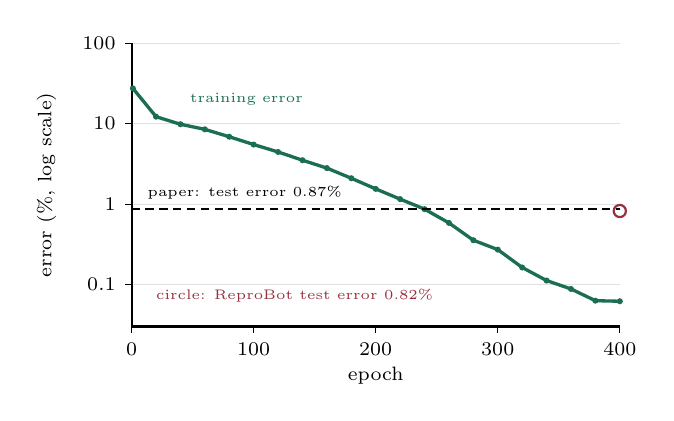
\begin{tikzpicture}
  \draw[black!12] (0,0.534) -- (6.2,0.534);
  \draw (0,0.534) -- (-0.08,0.534) node[left, font=\scriptsize] {0.1};
  \draw[black!12] (0,1.556) -- (6.2,1.556);
  \draw (0,1.556) -- (-0.08,1.556) node[left, font=\scriptsize] {1};
  \draw[black!12] (0,2.578) -- (6.2,2.578);
  \draw (0,2.578) -- (-0.08,2.578) node[left, font=\scriptsize] {10};
  \draw[black!12] (0,3.600) -- (6.2,3.600);
  \draw (0,3.600) -- (-0.08,3.600) node[left, font=\scriptsize] {100};
  \draw (0.000,0) -- (0.000,-0.08) node[below, font=\scriptsize] {0};
  \draw (1.550,0) -- (1.550,-0.08) node[below, font=\scriptsize] {100};
  \draw (3.100,0) -- (3.100,-0.08) node[below, font=\scriptsize] {200};
  \draw (4.650,0) -- (4.650,-0.08) node[below, font=\scriptsize] {300};
  \draw (6.200,0) -- (6.200,-0.08) node[below, font=\scriptsize] {400};
  \draw[thick] (0,0) -- (6.2,0);
  \draw[thick] (0,0) -- (0,3.6);
  \node[font=\scriptsize] at (3.100,-0.62) {epoch};
  \node[font=\scriptsize, rotate=90] at (-1.08,1.800) {error (\%, log scale)};
  \draw[builtc, very thick] (0.016,3.026) -- (0.310,2.666) -- (0.620,2.570) -- (0.930,2.505) -- (1.240,2.411) -- (1.550,2.312) -- (1.860,2.218) -- (2.170,2.113) -- (2.480,2.013) -- (2.790,1.884) -- (3.100,1.749) -- (3.410,1.619) -- (3.720,1.492) -- (4.030,1.317) -- (4.340,1.097) -- (4.650,0.978) -- (4.960,0.751) -- (5.270,0.585) -- (5.580,0.478) -- (5.890,0.329) -- (6.200,0.322);
  \fill[builtc] (0.016,3.026) circle (1.1pt);
  \fill[builtc] (0.310,2.666) circle (1.1pt);
  \fill[builtc] (0.620,2.570) circle (1.1pt);
  \fill[builtc] (0.930,2.505) circle (1.1pt);
  \fill[builtc] (1.240,2.411) circle (1.1pt);
  \fill[builtc] (1.550,2.312) circle (1.1pt);
  \fill[builtc] (1.860,2.218) circle (1.1pt);
  \fill[builtc] (2.170,2.113) circle (1.1pt);
  \fill[builtc] (2.480,2.013) circle (1.1pt);
  \fill[builtc] (2.790,1.884) circle (1.1pt);
  \fill[builtc] (3.100,1.749) circle (1.1pt);
  \fill[builtc] (3.410,1.619) circle (1.1pt);
  \fill[builtc] (3.720,1.492) circle (1.1pt);
  \fill[builtc] (4.030,1.317) circle (1.1pt);
  \fill[builtc] (4.340,1.097) circle (1.1pt);
  \fill[builtc] (4.650,0.978) circle (1.1pt);
  \fill[builtc] (4.960,0.751) circle (1.1pt);
  \fill[builtc] (5.270,0.585) circle (1.1pt);
  \fill[builtc] (5.580,0.478) circle (1.1pt);
  \fill[builtc] (5.890,0.329) circle (1.1pt);
  \fill[builtc] (6.200,0.322) circle (1.1pt);
  \draw[black, densely dashed] (0,1.494) -- (6.2,1.494);
  \node[font=\tiny, anchor=south west, text=black] at (0.080,1.494) {paper: test error 0.87\%};
  \draw[missingc, thick] (6.200,1.468) circle (2.2pt);
  \node[font=\tiny, text=missingc, anchor=south west] at (0.186,0.180)
    {circle: ReproBot test error 0.82\%};
  \node[font=\tiny, text=builtc, anchor=west] at (0.620,2.886) {training error};
\end{tikzpicture}}\\[-1pt]
{\small (a) MLP with L2-SVM loss, MNIST}
\end{minipage}
\hfill
\begin{minipage}[t]{0.49\linewidth}\centering
\resizebox{0.97\linewidth}{!}{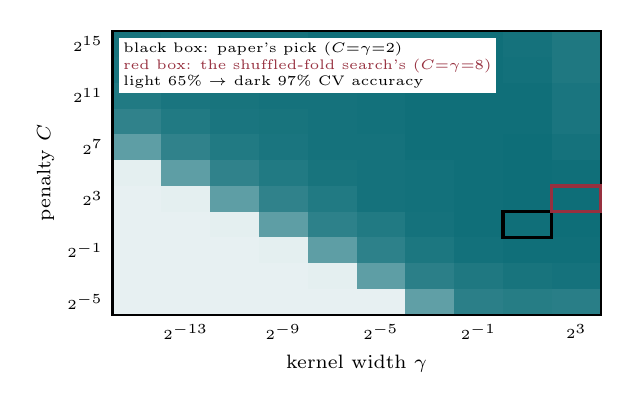
\begin{tikzpicture}
  \fill[loopc!10!white] (0.000,0.000) rectangle (0.620,0.327);
  \fill[loopc!10!white] (0.620,0.000) rectangle (1.240,0.327);
  \fill[loopc!10!white] (1.240,0.000) rectangle (1.860,0.327);
  \fill[loopc!10!white] (1.860,0.000) rectangle (2.480,0.327);
  \fill[loopc!10!white] (2.480,0.000) rectangle (3.100,0.327);
  \fill[loopc!10!white] (3.100,0.000) rectangle (3.720,0.327);
  \fill[loopc!66!white] (3.720,0.000) rectangle (4.340,0.327);
  \fill[loopc!88!white] (4.340,0.000) rectangle (4.960,0.327);
  \fill[loopc!90!white] (4.960,0.000) rectangle (5.580,0.327);
  \fill[loopc!89!white] (5.580,0.000) rectangle (6.200,0.327);
  \fill[loopc!10!white] (0.000,0.327) rectangle (0.620,0.655);
  \fill[loopc!10!white] (0.620,0.327) rectangle (1.240,0.655);
  \fill[loopc!10!white] (1.240,0.327) rectangle (1.860,0.655);
  \fill[loopc!10!white] (1.860,0.327) rectangle (2.480,0.655);
  \fill[loopc!11!white] (2.480,0.327) rectangle (3.100,0.655);
  \fill[loopc!67!white] (3.100,0.327) rectangle (3.720,0.655);
  \fill[loopc!88!white] (3.720,0.327) rectangle (4.340,0.655);
  \fill[loopc!93!white] (4.340,0.327) rectangle (4.960,0.655);
  \fill[loopc!96!white] (4.960,0.327) rectangle (5.580,0.655);
  \fill[loopc!97!white] (5.580,0.327) rectangle (6.200,0.655);
  \fill[loopc!10!white] (0.000,0.655) rectangle (0.620,0.982);
  \fill[loopc!10!white] (0.620,0.655) rectangle (1.240,0.982);
  \fill[loopc!10!white] (1.240,0.655) rectangle (1.860,0.982);
  \fill[loopc!11!white] (1.860,0.655) rectangle (2.480,0.982);
  \fill[loopc!67!white] (2.480,0.655) rectangle (3.100,0.982);
  \fill[loopc!87!white] (3.100,0.655) rectangle (3.720,0.982);
  \fill[loopc!94!white] (3.720,0.655) rectangle (4.340,0.982);
  \fill[loopc!98!white] (4.340,0.655) rectangle (4.960,0.982);
  \fill[loopc!99!white] (4.960,0.655) rectangle (5.580,0.982);
  \fill[loopc!99!white] (5.580,0.655) rectangle (6.200,0.982);
  \fill[loopc!10!white] (0.000,0.982) rectangle (0.620,1.309);
  \fill[loopc!10!white] (0.620,0.982) rectangle (1.240,1.309);
  \fill[loopc!11!white] (1.240,0.982) rectangle (1.860,1.309);
  \fill[loopc!67!white] (1.860,0.982) rectangle (2.480,1.309);
  \fill[loopc!87!white] (2.480,0.982) rectangle (3.100,1.309);
  \fill[loopc!92!white] (3.100,0.982) rectangle (3.720,1.309);
  \fill[loopc!97!white] (3.720,0.982) rectangle (4.340,1.309);
  \fill[loopc!99!white] (4.340,0.982) rectangle (4.960,1.309);
  \fill[loopc!99!white] (4.960,0.982) rectangle (5.580,1.309);
  \fill[loopc!100!white] (5.580,0.982) rectangle (6.200,1.309);
  \fill[loopc!10!white] (0.000,1.309) rectangle (0.620,1.636);
  \fill[loopc!11!white] (0.620,1.309) rectangle (1.240,1.636);
  \fill[loopc!67!white] (1.240,1.309) rectangle (1.860,1.636);
  \fill[loopc!86!white] (1.860,1.309) rectangle (2.480,1.636);
  \fill[loopc!92!white] (2.480,1.309) rectangle (3.100,1.636);
  \fill[loopc!97!white] (3.100,1.309) rectangle (3.720,1.636);
  \fill[loopc!98!white] (3.720,1.309) rectangle (4.340,1.636);
  \fill[loopc!99!white] (4.340,1.309) rectangle (4.960,1.636);
  \fill[loopc!100!white] (4.960,1.309) rectangle (5.580,1.636);
  \fill[loopc!100!white] (5.580,1.309) rectangle (6.200,1.636);
  \fill[loopc!11!white] (0.000,1.636) rectangle (0.620,1.964);
  \fill[loopc!67!white] (0.620,1.636) rectangle (1.240,1.964);
  \fill[loopc!86!white] (1.240,1.636) rectangle (1.860,1.964);
  \fill[loopc!92!white] (1.860,1.636) rectangle (2.480,1.964);
  \fill[loopc!96!white] (2.480,1.636) rectangle (3.100,1.964);
  \fill[loopc!97!white] (3.100,1.636) rectangle (3.720,1.964);
  \fill[loopc!98!white] (3.720,1.636) rectangle (4.340,1.964);
  \fill[loopc!99!white] (4.340,1.636) rectangle (4.960,1.964);
  \fill[loopc!100!white] (4.960,1.636) rectangle (5.580,1.964);
  \fill[loopc!99!white] (5.580,1.636) rectangle (6.200,1.964);
  \fill[loopc!67!white] (0.000,1.964) rectangle (0.620,2.291);
  \fill[loopc!86!white] (0.620,1.964) rectangle (1.240,2.291);
  \fill[loopc!92!white] (1.240,1.964) rectangle (1.860,2.291);
  \fill[loopc!95!white] (1.860,1.964) rectangle (2.480,2.291);
  \fill[loopc!97!white] (2.480,1.964) rectangle (3.100,2.291);
  \fill[loopc!97!white] (3.100,1.964) rectangle (3.720,2.291);
  \fill[loopc!99!white] (3.720,1.964) rectangle (4.340,2.291);
  \fill[loopc!99!white] (4.340,1.964) rectangle (4.960,2.291);
  \fill[loopc!100!white] (4.960,1.964) rectangle (5.580,2.291);
  \fill[loopc!97!white] (5.580,1.964) rectangle (6.200,2.291);
  \fill[loopc!86!white] (0.000,2.291) rectangle (0.620,2.618);
  \fill[loopc!92!white] (0.620,2.291) rectangle (1.240,2.618);
  \fill[loopc!95!white] (1.240,2.291) rectangle (1.860,2.618);
  \fill[loopc!96!white] (1.860,2.291) rectangle (2.480,2.618);
  \fill[loopc!97!white] (2.480,2.291) rectangle (3.100,2.618);
  \fill[loopc!98!white] (3.100,2.291) rectangle (3.720,2.618);
  \fill[loopc!99!white] (3.720,2.291) rectangle (4.340,2.618);
  \fill[loopc!99!white] (4.340,2.291) rectangle (4.960,2.618);
  \fill[loopc!99!white] (4.960,2.291) rectangle (5.580,2.618);
  \fill[loopc!95!white] (5.580,2.291) rectangle (6.200,2.618);
  \fill[loopc!92!white] (0.000,2.618) rectangle (0.620,2.945);
  \fill[loopc!95!white] (0.620,2.618) rectangle (1.240,2.945);
  \fill[loopc!96!white] (1.240,2.618) rectangle (1.860,2.945);
  \fill[loopc!97!white] (1.860,2.618) rectangle (2.480,2.945);
  \fill[loopc!97!white] (2.480,2.618) rectangle (3.100,2.945);
  \fill[loopc!98!white] (3.100,2.618) rectangle (3.720,2.945);
  \fill[loopc!99!white] (3.720,2.618) rectangle (4.340,2.945);
  \fill[loopc!99!white] (4.340,2.618) rectangle (4.960,2.945);
  \fill[loopc!99!white] (4.960,2.618) rectangle (5.580,2.945);
  \fill[loopc!95!white] (5.580,2.618) rectangle (6.200,2.945);
  \fill[loopc!95!white] (0.000,2.945) rectangle (0.620,3.273);
  \fill[loopc!95!white] (0.620,2.945) rectangle (1.240,3.273);
  \fill[loopc!95!white] (1.240,2.945) rectangle (1.860,3.273);
  \fill[loopc!97!white] (1.860,2.945) rectangle (2.480,3.273);
  \fill[loopc!98!white] (2.480,2.945) rectangle (3.100,3.273);
  \fill[loopc!99!white] (3.100,2.945) rectangle (3.720,3.273);
  \fill[loopc!99!white] (3.720,2.945) rectangle (4.340,3.273);
  \fill[loopc!99!white] (4.340,2.945) rectangle (4.960,3.273);
  \fill[loopc!98!white] (4.960,2.945) rectangle (5.580,3.273);
  \fill[loopc!93!white] (5.580,2.945) rectangle (6.200,3.273);
  \fill[loopc!96!white] (0.000,3.273) rectangle (0.620,3.600);
  \fill[loopc!95!white] (0.620,3.273) rectangle (1.240,3.600);
  \fill[loopc!97!white] (1.240,3.273) rectangle (1.860,3.600);
  \fill[loopc!97!white] (1.860,3.273) rectangle (2.480,3.600);
  \fill[loopc!99!white] (2.480,3.273) rectangle (3.100,3.600);
  \fill[loopc!99!white] (3.100,3.273) rectangle (3.720,3.600);
  \fill[loopc!99!white] (3.720,3.273) rectangle (4.340,3.600);
  \fill[loopc!99!white] (4.340,3.273) rectangle (4.960,3.600);
  \fill[loopc!97!white] (4.960,3.273) rectangle (5.580,3.600);
  \fill[loopc!93!white] (5.580,3.273) rectangle (6.200,3.600);
  \draw[thick] (0,0) rectangle (6.2,3.6);
  \node[font=\tiny, below] at (0.930,0) {$2^{-13}$};
  \node[font=\tiny, below] at (2.170,0) {$2^{-9}$};
  \node[font=\tiny, below] at (3.410,0) {$2^{-5}$};
  \node[font=\tiny, below] at (4.650,0) {$2^{-1}$};
  \node[font=\tiny, below] at (5.890,0) {$2^{3}$};
  \node[font=\tiny, left] at (0,0.164) {$2^{-5}$};
  \node[font=\tiny, left] at (0,0.818) {$2^{-1}$};
  \node[font=\tiny, left] at (0,1.473) {$2^{3}$};
  \node[font=\tiny, left] at (0,2.127) {$2^{7}$};
  \node[font=\tiny, left] at (0,2.782) {$2^{11}$};
  \node[font=\tiny, left] at (0,3.436) {$2^{15}$};
  \draw[black, very thick] (4.960,0.982)
    rectangle (5.580,1.309);
  \draw[missingc, very thick] (5.580,1.309)
    rectangle (6.200,1.636);
  \node[font=\scriptsize] at (3.100,-0.62) {kernel width $\gamma$};
  \node[font=\scriptsize, rotate=90] at (-0.85,1.800) {penalty $C$};
  \node[font=\tiny, anchor=north west, fill=white, inner sep=1.5pt, align=left]
    at (0.08,3.520)
    {black box: paper's pick ($C{=}\gamma{=}2$)\\
      \textcolor{missingc}{red box: the shuffled-fold search's ($C{=}\gamma{=}8$)}\\
      light 65\% $\to$ dark 97\% CV accuracy};
\end{tikzpicture}}\\[-1pt]
{\small (b) RBF SVM model selection, svmguide1}
\end{minipage}
\\[10pt]
\begin{minipage}[t]{0.49\linewidth}\centering
\resizebox{0.97\linewidth}{!}{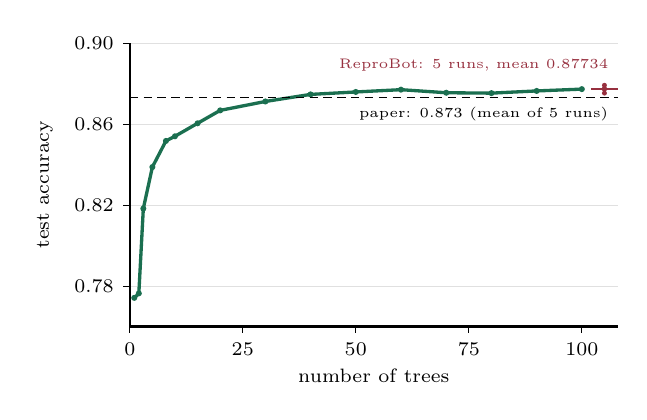
\begin{tikzpicture}
  \draw[black!12] (0,0.514) -- (6.2,0.514);
  \draw (0,0.514) -- (-0.08,0.514) node[left, font=\scriptsize] {0.78};
  \draw[black!12] (0,1.543) -- (6.2,1.543);
  \draw (0,1.543) -- (-0.08,1.543) node[left, font=\scriptsize] {0.82};
  \draw[black!12] (0,2.571) -- (6.2,2.571);
  \draw (0,2.571) -- (-0.08,2.571) node[left, font=\scriptsize] {0.86};
  \draw[black!12] (0,3.600) -- (6.2,3.600);
  \draw (0,3.600) -- (-0.08,3.600) node[left, font=\scriptsize] {0.90};
  \draw (0.000,0) -- (0.000,-0.08) node[below, font=\scriptsize] {0};
  \draw (1.435,0) -- (1.435,-0.08) node[below, font=\scriptsize] {25};
  \draw (2.870,0) -- (2.870,-0.08) node[below, font=\scriptsize] {50};
  \draw (4.306,0) -- (4.306,-0.08) node[below, font=\scriptsize] {75};
  \draw (5.741,0) -- (5.741,-0.08) node[below, font=\scriptsize] {100};
  \draw[thick] (0,0) -- (6.2,0);
  \draw[thick] (0,0) -- (0,3.6);
  \node[font=\scriptsize] at (3.100,-0.62) {number of trees};
  \node[font=\scriptsize, rotate=90] at (-1.08,1.800) {test accuracy};
  \draw[builtc, very thick] (0.057,0.365) -- (0.115,0.422) -- (0.172,1.499) -- (0.287,2.026) -- (0.459,2.358) -- (0.574,2.417) -- (0.861,2.582) -- (1.148,2.746) -- (1.722,2.859) -- (2.296,2.949) -- (2.870,2.980) -- (3.444,3.009) -- (4.019,2.970) -- (4.593,2.965) -- (5.167,2.993) -- (5.741,3.016);
  \fill[builtc] (0.057,0.365) circle (1.1pt);
  \fill[builtc] (0.115,0.422) circle (1.1pt);
  \fill[builtc] (0.172,1.499) circle (1.1pt);
  \fill[builtc] (0.287,2.026) circle (1.1pt);
  \fill[builtc] (0.459,2.358) circle (1.1pt);
  \fill[builtc] (0.574,2.417) circle (1.1pt);
  \fill[builtc] (0.861,2.582) circle (1.1pt);
  \fill[builtc] (1.148,2.746) circle (1.1pt);
  \fill[builtc] (1.722,2.859) circle (1.1pt);
  \fill[builtc] (2.296,2.949) circle (1.1pt);
  \fill[builtc] (2.870,2.980) circle (1.1pt);
  \fill[builtc] (3.444,3.009) circle (1.1pt);
  \fill[builtc] (4.019,2.970) circle (1.1pt);
  \fill[builtc] (4.593,2.965) circle (1.1pt);
  \fill[builtc] (5.167,2.993) circle (1.1pt);
  \fill[builtc] (5.741,3.016) circle (1.1pt);
  \draw[black, densely dashed] (0,2.906) -- (6.2,2.906);
  \node[font=\tiny, anchor=north east, text=black] at (6.200,2.906) {paper: 0.873 (mean of 5 runs)};
  \fill[missingc] (6.028,3.016) circle (0.9pt);
  \fill[missingc] (6.028,3.019) circle (0.9pt);
  \fill[missingc] (6.028,2.965) circle (0.9pt);
  \fill[missingc] (6.028,3.065) circle (0.9pt);
  \fill[missingc] (6.028,3.021) circle (0.9pt);
  \draw[missingc, thick] (5.856,3.017) -- (6.200,3.017);
  \node[font=\tiny, text=missingc, anchor=south east] at (6.200,3.115)
    {ReproBot: 5 runs, mean 0.87734};
\end{tikzpicture}}\\[-1pt]
{\small (c) Random forest, Fashion-MNIST}
\end{minipage}
\hfill
\begin{minipage}[t]{0.49\linewidth}\centering
\resizebox{0.97\linewidth}{!}{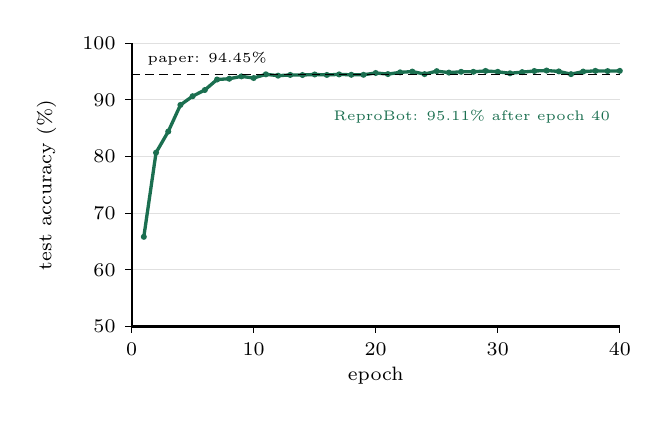
\begin{tikzpicture}
  \draw[black!12] (0,0.000) -- (6.2,0.000);
  \draw (0,0.000) -- (-0.08,0.000) node[left, font=\scriptsize] {50};
  \draw[black!12] (0,0.720) -- (6.2,0.720);
  \draw (0,0.720) -- (-0.08,0.720) node[left, font=\scriptsize] {60};
  \draw[black!12] (0,1.440) -- (6.2,1.440);
  \draw (0,1.440) -- (-0.08,1.440) node[left, font=\scriptsize] {70};
  \draw[black!12] (0,2.160) -- (6.2,2.160);
  \draw (0,2.160) -- (-0.08,2.160) node[left, font=\scriptsize] {80};
  \draw[black!12] (0,2.880) -- (6.2,2.880);
  \draw (0,2.880) -- (-0.08,2.880) node[left, font=\scriptsize] {90};
  \draw[black!12] (0,3.600) -- (6.2,3.600);
  \draw (0,3.600) -- (-0.08,3.600) node[left, font=\scriptsize] {100};
  \draw (0.000,0) -- (0.000,-0.08) node[below, font=\scriptsize] {0};
  \draw (1.550,0) -- (1.550,-0.08) node[below, font=\scriptsize] {10};
  \draw (3.100,0) -- (3.100,-0.08) node[below, font=\scriptsize] {20};
  \draw (4.650,0) -- (4.650,-0.08) node[below, font=\scriptsize] {30};
  \draw (6.200,0) -- (6.200,-0.08) node[below, font=\scriptsize] {40};
  \draw[thick] (0,0) -- (6.2,0);
  \draw[thick] (0,0) -- (0,3.6);
  \node[font=\scriptsize] at (3.100,-0.62) {epoch};
  \node[font=\scriptsize, rotate=90] at (-1.08,1.800) {test accuracy (\%)};
  \draw[builtc, very thick] (0.155,1.140) -- (0.310,2.209) -- (0.465,2.477) -- (0.620,2.815) -- (0.775,2.926) -- (0.930,3.005) -- (1.085,3.138) -- (1.240,3.148) -- (1.395,3.178) -- (1.550,3.157) -- (1.705,3.204) -- (1.860,3.187) -- (2.015,3.196) -- (2.170,3.195) -- (2.325,3.202) -- (2.480,3.196) -- (2.635,3.203) -- (2.790,3.198) -- (2.945,3.198) -- (3.100,3.221) -- (3.255,3.207) -- (3.410,3.229) -- (3.565,3.239) -- (3.720,3.207) -- (3.875,3.244) -- (4.030,3.226) -- (4.185,3.236) -- (4.340,3.236) -- (4.495,3.247) -- (4.650,3.236) -- (4.805,3.217) -- (4.960,3.232) -- (5.115,3.246) -- (5.270,3.252) -- (5.425,3.241) -- (5.580,3.206) -- (5.735,3.239) -- (5.890,3.248) -- (6.045,3.245) -- (6.200,3.248);
  \fill[builtc] (0.155,1.140) circle (1.1pt);
  \fill[builtc] (0.310,2.209) circle (1.1pt);
  \fill[builtc] (0.465,2.477) circle (1.1pt);
  \fill[builtc] (0.620,2.815) circle (1.1pt);
  \fill[builtc] (0.775,2.926) circle (1.1pt);
  \fill[builtc] (0.930,3.005) circle (1.1pt);
  \fill[builtc] (1.085,3.138) circle (1.1pt);
  \fill[builtc] (1.240,3.148) circle (1.1pt);
  \fill[builtc] (1.395,3.178) circle (1.1pt);
  \fill[builtc] (1.550,3.157) circle (1.1pt);
  \fill[builtc] (1.705,3.204) circle (1.1pt);
  \fill[builtc] (1.860,3.187) circle (1.1pt);
  \fill[builtc] (2.015,3.196) circle (1.1pt);
  \fill[builtc] (2.170,3.195) circle (1.1pt);
  \fill[builtc] (2.325,3.202) circle (1.1pt);
  \fill[builtc] (2.480,3.196) circle (1.1pt);
  \fill[builtc] (2.635,3.203) circle (1.1pt);
  \fill[builtc] (2.790,3.198) circle (1.1pt);
  \fill[builtc] (2.945,3.198) circle (1.1pt);
  \fill[builtc] (3.100,3.221) circle (1.1pt);
  \fill[builtc] (3.255,3.207) circle (1.1pt);
  \fill[builtc] (3.410,3.229) circle (1.1pt);
  \fill[builtc] (3.565,3.239) circle (1.1pt);
  \fill[builtc] (3.720,3.207) circle (1.1pt);
  \fill[builtc] (3.875,3.244) circle (1.1pt);
  \fill[builtc] (4.030,3.226) circle (1.1pt);
  \fill[builtc] (4.185,3.236) circle (1.1pt);
  \fill[builtc] (4.340,3.236) circle (1.1pt);
  \fill[builtc] (4.495,3.247) circle (1.1pt);
  \fill[builtc] (4.650,3.236) circle (1.1pt);
  \fill[builtc] (4.805,3.217) circle (1.1pt);
  \fill[builtc] (4.960,3.232) circle (1.1pt);
  \fill[builtc] (5.115,3.246) circle (1.1pt);
  \fill[builtc] (5.270,3.252) circle (1.1pt);
  \fill[builtc] (5.425,3.241) circle (1.1pt);
  \fill[builtc] (5.580,3.206) circle (1.1pt);
  \fill[builtc] (5.735,3.239) circle (1.1pt);
  \fill[builtc] (5.890,3.248) circle (1.1pt);
  \fill[builtc] (6.045,3.245) circle (1.1pt);
  \fill[builtc] (6.200,3.248) circle (1.1pt);
  \draw[black, densely dashed] (0,3.200) -- (6.2,3.200);
  \node[font=\tiny, anchor=south west, text=black] at (0.080,3.200) {paper: 94.45\%};
  \node[font=\tiny, text=builtc, anchor=east] at (6.200,2.664)
    {ReproBot: 95.11\% after epoch 40};
\end{tikzpicture}}\\[-1pt]
{\small (d) Soft decision tree, MNIST}
\end{minipage}
\caption{Four of the five generated implementations at the papers' own full settings, with each
paper's reported result as a dashed line. (a) Training error per 20 epochs, log scale; the circle
is the reproduced test error, evaluated once at the end. (b) Five-fold cross-validation accuracy
over the SVM's $(C, \gamma)$ grid, with the paper's own setting and the shuffled-fold search's
pick outlined. (c) Test accuracy as trees are added, for the first of five repetitions, with all
five repetitions' final accuracies at the right. (d) Test accuracy per epoch. Panels (b) and (c)
were computed with the generated scripts' own configuration and code; all other points are read
directly from the run logs.}
\label{fig:curves}
\end{figure*}


Two of the five needed a human correction before their final run, and the report says which:
Tang's unstated SVM penalty was changed from the common default $C = 1.0$ to $C = 0.1$ after a
six-configuration ablation, and the soft-tree paper's misprinted loss was implemented as its
evident intent. Both are in Table~\ref{tab:problems}. The other three ran unassisted.

\textbf{Tang: an MLP with a margin loss.} The network trained for the paper's own 400 epochs,
training error falling to 0.062\% (Figure~\ref{fig:curves}a), and the test set --- evaluated once,
at the end --- gave 0.82\% against the paper's 0.87\%: five test images out of 10{,}000, well
inside the $\pm$0.1857 that binomial noise on a 10{,}000-image test set allows.

\textbf{The SVM guide: the cleanest exactness test available.} Because scikit-learn's
\texttt{SVC} wraps the same LIBSVM the guide itself used, the library \emph{is} the method, and
at the paper's own settings the reproduction matches its reported accuracies exactly
(Table~\ref{tab:svmexact}). Everything that remains is model selection:
Figure~\ref{fig:curves}b shows the cross-validation surface the generated script searched, with a
broad ridge of settings above 96\% and the paper's own choice one cell away from the search's.

\begin{table}[tbp]
\centering
\small
\caption{svmguide1 test accuracy. The paper's three reported settings are reproduced exactly by
scikit-learn's \texttt{SVC}, because it wraps the same LIBSVM implementation. Only the grid
search's choice differs. Paper values read from the PDF itself.}
\label{tab:svmexact}
\squeeze
\begin{tabular}{L{0.42\linewidth}rr}
\toprule
Setting & Paper & ReproBot \\
\midrule
Unscaled features, library defaults & 66.925\% & 66.925\% \\
Scaled to $[-1,1]$, library defaults & 96.15\% & 96.15\% \\
Scaled, $C = 2$, $\gamma = 2$ & 96.875\% & 96.875\% \\
Scaled, the paper's full grid-search procedure & 96.9\% & 96.625 -- 96.925\% \\
\bottomrule
\end{tabular}
\end{table}

\textbf{Fashion-MNIST: a claim that is already an average.} The paper reports the mean of five
runs with shuffled training data, so the generated script performs five runs and reports all
five: 0.8773, 0.8774, 0.8753, 0.8792 and 0.8775, mean 0.87734 against the claimed 0.873. That
measured spread is what gives this row the tightest tolerance in the table, $\pm$0.00175 --- and
the reproduction still clears it on the high side. Figure~\ref{fig:curves}c shows why 100 trees
was a safe choice: accuracy is already on its plateau by 30.

\textbf{The soft decision tree: an under-specified paper reproduced through disclosed guesses.}
The paper states the tree's depth and essentially nothing else about training, so the generated
script chose and recorded a value for each missing setting. Test accuracy passed the paper's
94.45\% at epoch 11 and finished at 95.11\% (Figure~\ref{fig:curves}d). No setting was chosen on
the test set, so a result 0.7 points above the claim with every guess disclosed is a comfortable
reproduction rather than a lucky one.

\textbf{Wijaya: the one that needed more than one run.} The first full run of the housing-price
network gave test RMSE 3.1285 against the claimed 3.02 --- worse than the claim, with no noise
model to say whether that mattered. The Critic returned \texttt{inconclusive} and asked for
seeds instead of ruling. Two more full runs gave 3.0283 and 2.9520, and the re-judgement was
\texttt{pass} at a mean of 3.03629 with a tolerance of $\pm$0.2044 that was now measured rather
than assumed. A system that ruled on one number would have called this paper a failure at 3.13,
or a success at 2.76, depending only on which run you happened to see.

\subsection{Repeatability: three papers, three runs each, PDF to report}
\label{sec:repeat}

A single successful run proves little, so three of the papers were run three times each, from the
PDF through to a rendered report, with the whole loop switched on: retries, live check-ups, the
Critic's verdict, its seed escalation and its guided fidelity retry. Each paper was re-read from
its PDF the same day, so no extraction was inherited from an earlier session.

\textbf{9 of 9 runs reproduced their claim, and every run reached \texttt{full} on its first
attempt} --- no retry was consumed. End-to-end wall clock was 77 to 238 seconds per run, so the
whole batch cost about 35 minutes of laptop CPU.

\begin{table*}[tbp]
\centering
\small
\caption{Three papers, three independent runs each, 2026-10-09. The claim is pinned by id,
because target-claim selection is not reproducible across Reader runs. The last column is the
finding: each paper's spread has exactly one named cause.}
\label{tab:repeat}
\squeeze
\begin{tabular}{L{0.17\textwidth}L{0.09\textwidth}cL{0.07\textwidth}L{0.07\textwidth}L{0.07\textwidth}L{0.29\textwidth}}
\toprule
Paper & Claim & Passes & Run 1 & Run 2 & Run 3 & Why the runs differ \\
\midrule
SVM guide (\texttt{c2}) & 96.9\% & \textbf{3/3} & 96.625 & 96.925 & 96.625 & The paper says
  ``five-fold cross-validation'' and never says whether the folds are shuffled \\
Fashion-MNIST (\texttt{c41}) & 0.873 & \textbf{3/3} & 0.87734 & 0.87734 & 0.87734 & Nothing --- the
  protocol is fully specified \\
Wijaya (\texttt{c3}) & RMSE 3.02 & \textbf{3/3} & 2.76299 & 2.86305 & 3.03629$^{*}$ & The paper
  gives the 405/101 split sizes and never says how rows are assigned \\
\bottomrule
\end{tabular}
\\[2pt]
{\small $^{*}$ Run 3 is the mean of three seeds. Its first value, 3.1285, was judged
\texttt{inconclusive} and the Critic escalated on its own.}
\end{table*}

\subsection{Run-to-run variance is a property of the paper}
\label{sec:unstated}

This is the finding we would keep if we could keep only one. Across the nine runs, \textbf{every
disagreement between two runs of the same paper traced to exactly one detail that paper never
states, and in every case we could name it.} Table~\ref{tab:unstated} gives the mechanism for
each, and Figure~\ref{fig:spread} plots every reproduced value this project holds for the two
papers it ran most often.

\begin{table*}[tbp]
\centering
\small
\caption{The mechanism behind each paper's spread. Variance here is not noise in the system; it
is the paper's own under-specification, made visible and named.}
\label{tab:unstated}
\squeeze
\begin{tabular}{L{0.14\textwidth}L{0.24\textwidth}L{0.25\textwidth}L{0.24\textwidth}}
\toprule
Paper & What the paper does not state & What that changes & Observed consequence \\
\midrule
Fashion-MNIST & Nothing relevant: official 60k/10k split, raw pixels, 100 trees, entropy
  criterion, depth 100, five repetitions with shuffled data & --- & Three independently generated
  scripts of 303, 274 and 291 lines --- 299 and 290 changed lines against the first --- produced
  \textbf{bit-identical} values. All three independently chose base seed 42, per-repetition
  \texttt{seed + i}, and \texttt{random\_state=rep\_seed} on both the shuffle and the forest \\
SVM guide & Whether the five cross-validation folds are shuffled & Which $(C, \gamma)$ the grid
  search selects, and therefore the test accuracy & Runs 1 and 3 shuffled with seed 42, selected
  $C{=}8, \gamma{=}8$ at CV 96.9894\% and scored 96.625\% --- identically. Run 2 used
  scikit-learn's unshuffled contiguous folds, selected $C{=}2, \gamma{=}8$ at a \emph{lower} CV of
  96.7952\%, and scored \textbf{96.925\%} \\
Wijaya & How the 405/101 split is drawn & Which rows are held out of a 506-row dataset & The RMSE
  moves continuously: 2.76299, 2.86305, 3.03629 across three runs, and 2.619 to 4.003 across five
  independent generations \\
\bottomrule
\end{tabular}
\end{table*}


\begin{figure*}[tbp]
\centering
\begin{minipage}[t]{0.49\linewidth}\centering
\resizebox{0.97\linewidth}{!}{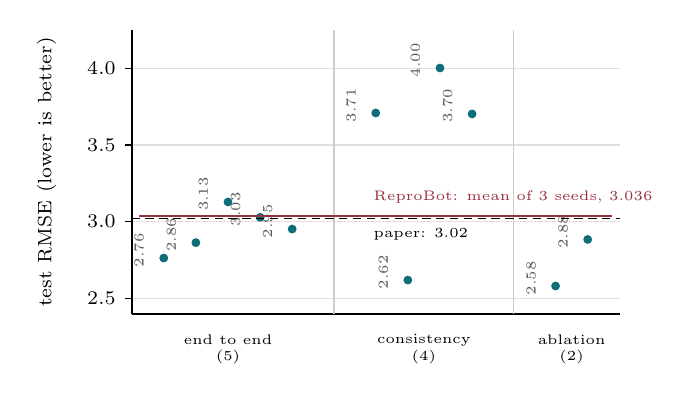
\begin{tikzpicture}
  \draw[black!12] (0,0.195) -- (6.2,0.195);
  \draw (0,0.195) -- (-0.08,0.195) node[left, font=\scriptsize] {2.5};
  \draw[black!12] (0,1.168) -- (6.2,1.168);
  \draw (0,1.168) -- (-0.08,1.168) node[left, font=\scriptsize] {3.0};
  \draw[black!12] (0,2.141) -- (6.2,2.141);
  \draw (0,2.141) -- (-0.08,2.141) node[left, font=\scriptsize] {3.5};
  \draw[black!12] (0,3.114) -- (6.2,3.114);
  \draw (0,3.114) -- (-0.08,3.114) node[left, font=\scriptsize] {4.0};
  \draw[thick] (0,0) -- (6.2,0);
  \draw[thick] (0,0) -- (0,3.6);
  \node[font=\scriptsize] at (3.100,-0.62) {};
  \node[font=\scriptsize, rotate=90] at (-1.08,1.800) {test RMSE (lower is better)};
  \fill[loopc] (0.408,0.706) circle (1.6pt);
  \node[font=\tiny, text=black!65, anchor=south, rotate=90] at (0.278,0.806) {2.76};
  \fill[loopc] (0.816,0.901) circle (1.6pt);
  \node[font=\tiny, text=black!65, anchor=south, rotate=90] at (0.686,1.001) {2.86};
  \fill[loopc] (1.224,1.418) circle (1.6pt);
  \node[font=\tiny, text=black!65, anchor=south, rotate=90] at (1.094,1.518) {3.13};
  \fill[loopc] (1.632,1.223) circle (1.6pt);
  \node[font=\tiny, text=black!65, anchor=south, rotate=90] at (1.502,1.323) {3.03};
  \fill[loopc] (2.039,1.074) circle (1.6pt);
  \node[font=\tiny, text=black!65, anchor=south, rotate=90] at (1.909,1.174) {2.95};
  \node[font=\tiny, align=center, anchor=north] at (1.224,-0.14) {end to end\\(5)};
  \draw[black!20] (2.570,0) -- (2.570,3.6);
  \fill[loopc] (3.100,2.548) circle (1.6pt);
  \node[font=\tiny, text=black!65, anchor=south, rotate=90] at (2.970,2.648) {3.71};
  \fill[loopc] (3.508,0.426) circle (1.6pt);
  \node[font=\tiny, text=black!65, anchor=south, rotate=90] at (3.378,0.526) {2.62};
  \fill[loopc] (3.916,3.119) circle (1.6pt);
  \node[font=\tiny, text=black!65, anchor=south, rotate=90] at (3.786,3.219) {4.00};
  \fill[loopc] (4.324,2.536) circle (1.6pt);
  \node[font=\tiny, text=black!65, anchor=south, rotate=90] at (4.194,2.636) {3.70};
  \node[font=\tiny, align=center, anchor=north] at (3.712,-0.14) {consistency\\(4)};
  \draw[black!20] (4.854,0) -- (4.854,3.6);
  \fill[loopc] (5.384,0.351) circle (1.6pt);
  \node[font=\tiny, text=black!65, anchor=south, rotate=90] at (5.254,0.451) {2.58};
  \fill[loopc] (5.792,0.942) circle (1.6pt);
  \node[font=\tiny, text=black!65, anchor=south, rotate=90] at (5.662,1.042) {2.88};
  \node[font=\tiny, align=center, anchor=north] at (5.588,-0.14) {ablation\\(2)};
  \draw[black, densely dashed] (0,1.206) -- (6.2,1.206);
  \node[font=\tiny, anchor=north west, text=black] at (2.950,1.206) {paper: 3.02};
  \draw[missingc, thick] (0.1,1.238) -- (6.100,1.238);
  \node[font=\tiny, text=missingc, anchor=south west] at (2.950,1.278) {ReproBot: mean of 3 seeds, 3.036};
\end{tikzpicture}}\\[-1pt]
{\small (a) Wijaya 2023: the split is never stated}
\end{minipage}
\hfill
\begin{minipage}[t]{0.49\linewidth}\centering
\resizebox{0.97\linewidth}{!}{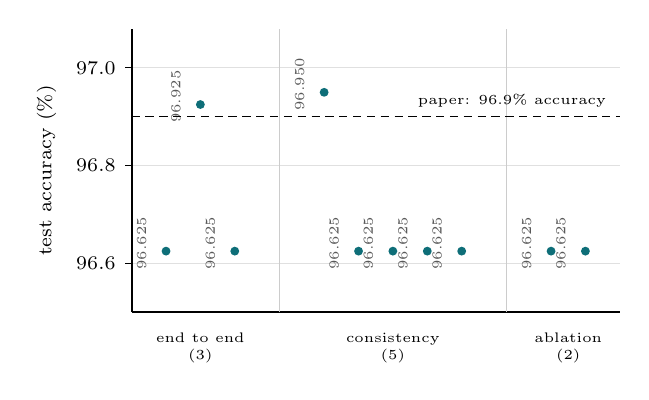
\begin{tikzpicture}
  \draw[black!12] (0,0.621) -- (6.2,0.621);
  \draw (0,0.621) -- (-0.08,0.621) node[left, font=\scriptsize] {96.6};
  \draw[black!12] (0,1.862) -- (6.2,1.862);
  \draw (0,1.862) -- (-0.08,1.862) node[left, font=\scriptsize] {96.8};
  \draw[black!12] (0,3.103) -- (6.2,3.103);
  \draw (0,3.103) -- (-0.08,3.103) node[left, font=\scriptsize] {97.0};
  \draw[thick] (0,0) -- (6.2,0);
  \draw[thick] (0,0) -- (0,3.6);
  \node[font=\scriptsize] at (3.100,-0.62) {};
  \node[font=\scriptsize, rotate=90] at (-1.08,1.800) {test accuracy (\%)};
  \fill[loopc] (0.437,0.776) circle (1.6pt);
  \node[font=\tiny, text=black!65, anchor=south, rotate=90] at (0.307,0.876) {96.625};
  \fill[loopc] (0.873,2.638) circle (1.6pt);
  \node[font=\tiny, text=black!65, anchor=south, rotate=90] at (0.743,2.738) {96.925};
  \fill[loopc] (1.310,0.776) circle (1.6pt);
  \node[font=\tiny, text=black!65, anchor=south, rotate=90] at (1.180,0.876) {96.625};
  \node[font=\tiny, align=center, anchor=north] at (0.873,-0.14) {end to end\\(3)};
  \draw[black!20] (1.877,0) -- (1.877,3.6);
  \fill[loopc] (2.445,2.793) circle (1.6pt);
  \node[font=\tiny, text=black!65, anchor=south, rotate=90] at (2.315,2.893) {96.950};
  \fill[loopc] (2.882,0.776) circle (1.6pt);
  \node[font=\tiny, text=black!65, anchor=south, rotate=90] at (2.752,0.876) {96.625};
  \fill[loopc] (3.318,0.776) circle (1.6pt);
  \node[font=\tiny, text=black!65, anchor=south, rotate=90] at (3.188,0.876) {96.625};
  \fill[loopc] (3.755,0.776) circle (1.6pt);
  \node[font=\tiny, text=black!65, anchor=south, rotate=90] at (3.625,0.876) {96.625};
  \fill[loopc] (4.192,0.776) circle (1.6pt);
  \node[font=\tiny, text=black!65, anchor=south, rotate=90] at (4.062,0.876) {96.625};
  \node[font=\tiny, align=center, anchor=north] at (3.318,-0.14) {consistency\\(5)};
  \draw[black!20] (4.759,0) -- (4.759,3.6);
  \fill[loopc] (5.327,0.776) circle (1.6pt);
  \node[font=\tiny, text=black!65, anchor=south, rotate=90] at (5.197,0.876) {96.625};
  \fill[loopc] (5.763,0.776) circle (1.6pt);
  \node[font=\tiny, text=black!65, anchor=south, rotate=90] at (5.633,0.876) {96.625};
  \node[font=\tiny, align=center, anchor=north] at (5.545,-0.14) {ablation\\(2)};
  \draw[black, densely dashed] (0,2.483) -- (6.2,2.483);
  \node[font=\tiny, anchor=south east, text=black] at (6.150,2.483) {paper: 96.9\% accuracy};
\end{tikzpicture}}\\[-1pt]
{\small (b) SVM guide: the fold shuffle is never stated}
\end{minipage}
\caption{Every reproduced value this project holds for the two papers it ran most often, grouped
by the experiment that produced it; the count in each group label is the number of runs. The
horizontal axis carries no quantity --- each run gets its own slot so nothing overlaps. (a) Wijaya
never states how its 405/101 split is drawn, so every generation draws its own and the RMSE moves
continuously; the red line is the judged mean of the three seeds the Critic escalated to. (b) The
SVM guide never states whether its five cross-validation folds are shuffled; every run that
shuffled them landed on 96.625\%, and the two that did not landed above the claim. Both papers'
claims sit inside their spread.}
\label{fig:spread}
\end{figure*}


\textbf{The SVM guide's mechanism is worth stating exactly, because it is counter-intuitive.}
The grid search optimises cross-validation accuracy, and here the cross-validation winner was the
test loser: the shuffled-fold run's choice won cross-validation by 0.19 points and lost on test by
0.30. Both runs pass, and both are faithful implementations of what the paper describes. The
paper's own answer, $C = \gamma = 2$, gives 96.9\%. One unstated word --- shuffled --- is the whole
difference.

\textbf{Fashion-MNIST's is worth stating because it is the control.} Three generations whose
texts barely resemble each other produced the same five numbers to four decimal places. When a
paper specifies its protocol completely, ReproBot's output is deterministic across generations.
That is the strongest available evidence that the variance seen elsewhere is not the Coder being
unreliable.

\subsection{Coverage: how much of each paper was tested}

A replication that targets one claim is fast and partial, and the reports say so.
Table~\ref{tab:coverage} gives the denominator: how many claims the Reader extracted from each
paper, how many distinct results remain after merging duplicates, and how many were actually
reproduced. Every generated report lists the untested remainder explicitly as \texttt{not tested}
rather than omitting it.

\begin{table}[tbp]
\centering
\small
\caption{Claims extracted against claims tested. Merging collapses one result printed in prose, a
table and a figure; it only bites where a paper repeats itself. A dash means merging was never run
for that paper.}
\label{tab:coverage}
\squeeze
\begin{tabular}{L{0.36\linewidth}rrr}
\toprule
Paper & Claims & Distinct & Tested \\
\midrule
Fashion-MNIST (2017) & 74 & 70 & 1 \\
Deep Residual Learning (2015) & 66 & --- & 0 \\
Wide Residual Networks (2016) & 61 & --- & 0 \\
SVM guide (2003) & 27 & 27 & 1 \\
All Convolutional Net (2014) & 17 & --- & 0 \\
Tang (2013) & 15 & 15 & 1 \\
Network In Network (2013) & 12 & --- & 0 \\
Frosst \& Hinton (2017) & 8 & 8 & 1 \\
Wijaya (2023) & 4 & 4 & 1 \\
\bottomrule
\end{tabular}
\end{table}

Claim counts are a property of a particular Reader run, not of the paper: an earlier extraction of
Wijaya found 14 claims that merged to 8 distinct results, where the run in the table found 4.
That instability is why every experiment in this report pins its target with
\texttt{-{}-claim-id} rather than letting the model choose again.

\subsection{Does the code match the paper? The Critic's review}

The verdict says whether the number matched; it cannot say whether the number was produced the
way the paper describes. A second Critic call reads the Reader extraction, the paper, the
line-numbered script, the Coder's recorded assumptions, the learning curve and a filtered runner
log, and returns findings --- each one a claim about the code with a paper quote and script lines
attached --- plus ranked hypotheses for any gap. Deterministic guards then decide what reaches the
Coder: a cited number must appear in the material, a paper quote must exist in the paper, script
lines and snippets must exist in the script, and a proposed fix may not introduce a technique the
paper never mentions. Findings that fail a guard are dropped, and the count of dropped findings is
printed in the report.

\begin{table}[tbp]
\centering
\small
\caption{Code review of the three end-to-end run-1 scripts, reviewer \texttt{claude-opus-5}. No
review reported a deviation from the paper or an implementation bug.}
\label{tab:review}
\squeeze
\begin{tabular}{L{0.26\linewidth}L{0.21\linewidth}L{0.17\linewidth}r}
\toprule
Paper & Fidelity & Deviations & Citations \\
\midrule
SVM guide & \texttt{faithful} & none & 10 / 10 \\
Fashion-MNIST & \texttt{faithful} & none & 8 / 8 \\
Wijaya & \texttt{faithful} & none & 12 / 15 \\
\bottomrule
\end{tabular}
\end{table}

Two things about Table~\ref{tab:review} are worth more than the ratings themselves. First, the
reviewer agreed with the arithmetic independently --- it read the code, not the verdict. Second,
the Wijaya review predicted its own result's direction without being told it: the unstated split
assignment, it wrote, ``can move test RMSE by several tenths, which plausibly explains the
reproduced 2.763 landing below the claimed 3.02.'' That is the same mechanism
Table~\ref{tab:unstated} names, arrived at from the code.

The reviewer is \texttt{claude-opus-5} on evidence, not preference. On a Wijaya script with a
deliberately swapped train/validation unpacking, Sonnet~5 missed the bug three times --- even with
the log stating the two split sizes --- and misdiagnosed it as a missing early-stopping rule,
which made the Coder add checkpoint selection that the paper never mentions. Opus found the swap,
the loop fixed it, and the next review returned \texttt{faithful}: a fidelity \texttt{fail} at
4.76 became a \texttt{pass} at 3.40 against 3.02, in eleven minutes.

\section{How a Verdict Is Made}
\label{sec:verdict}

The fidelity verdict is arithmetic. It makes no model call, opens no network connection and starts
no container, which means no model can argue its way to a pass:
\[
  \text{tolerance} = \max(2u,\ p),
\]
where $p$ is the claim's own reporting precision and $u$ the run's uncertainty. Precision is read
from the claim as printed: a claim of 3.02 is precise to $\pm 0.005$. Uncertainty comes from the
run itself where the run can supply it --- if two or more runs exist,
from their measured spread, as $\sigma\sqrt{2/n}$ when the claim is itself a mean and
$\sigma\sqrt{1 + 1/n}$ when a single-run claim is being compared with our mean --- and otherwise,
for an accuracy-like metric, from the binomial noise of a test set that size. When neither is
available there is no uncertainty estimate, and the band collapses to the claim's own precision.

Four verdicts follow, and each carries a consequence:

\begin{itemize}
  \item \texttt{pass} --- within tolerance, or better than the claim beyond it, which is recorded
    separately as \texttt{exceeds\_claim}.
  \item \texttt{fail} --- worse than the claim beyond tolerance, \emph{with} an uncertainty
    estimate. If the Critic's review found verified problems the paper itself states, this becomes
    a normal retry; otherwise it spends the single guided fidelity retry.
  \item \texttt{inconclusive} --- worse than the claim, but with no uncertainty estimate at all.
    The system asks for more seeds instead of ruling. This fired on Wijaya and changed the
    outcome.
  \item \texttt{not\_evaluated} --- nothing comparable: the run did not succeed, produced no value,
    stopped short of \texttt{full}, or targeted a claim the Reader does not have.
\end{itemize}

\begin{table}[tbp]
\centering
\small
\caption{Where each tolerance came from, and how wide it is relative to the claim. A tighter band
is a stronger pass. The two Wijaya rows are the same paper judged on one run and on three.}
\label{tab:tolerance}
\squeeze
\begin{tabular}{L{0.2\linewidth}L{0.31\linewidth}rr}
\toprule
Paper (claim) & Uncertainty source & Tolerance & of claim \\
\midrule
Fashion-MNIST (0.873) & Measured spread of 5 runs & $\pm$0.00175 & 0.20\% \\
SVM guide (96.9\%) & Binomial noise, 4{,}000 test rows & $\pm$0.5481 & 0.57\% \\
Soft tree (94.45\%) & Binomial noise, 10{,}000 test images & $\pm$0.4579 & 0.48\% \\
Tang (0.87\%) & Binomial noise, 10{,}000 test images & $\pm$0.1857 & 21\% \\
Wijaya (3.02), 1 run & None --- reporting precision only & $\pm$0.005 & 0.17\% \\
Wijaya (3.02), 3 seeds & Measured spread of 3 seeds & $\pm$0.2044 & 6.8\% \\
\bottomrule
\end{tabular}
\end{table}

Table~\ref{tab:tolerance} is the honesty column of this report. A \texttt{pass} at $\pm$0.00175 on
0.873 and a \texttt{pass} at $\pm$0.2044 on 3.02 are not the same statement, and a bare verdict
hides the difference. So the tolerance is printed everywhere the verdict appears, and when the
band exceeds 10\% of the claim the report adds an explicit warning. An earlier escalation of the
same Wijaya claim passed at a mean of 3.3292 with a tolerance of $\pm$1.0680 --- 35\% of the claim
--- and its report says in as many words that the result is \emph{consistent with} the paper rather
than a close match. Tang's $\pm$0.1857 on a claim of 0.87\% is the same situation in a different
guise: a test error that small is simply not measurable to better than about a fifth of itself on
10{,}000 images.

\section{The Three Experiments}
\label{sec:experiments}

Beyond the per-paper fidelity runs, three experiments were run to measure the system rather than
the papers. Table~\ref{tab:experiments} summarises them. Across all the runs this project holds,
32 carry a Critic verdict: 24 \texttt{pass}, 3 \texttt{inconclusive} and 5
\texttt{not\_evaluated} --- three cheap-stage runs, one generation that crashed at \texttt{probe},
and one ablation leg that never reached \texttt{full}.

\begin{table*}[tbp]
\centering
\small
\caption{The four measurements in this report, and what each one actually establishes.}
\label{tab:experiments}
\squeeze
\begin{tabular}{L{0.14\textwidth}L{0.22\textwidth}cL{0.48\textwidth}}
\toprule
Experiment & Design & Runs & Headline finding \\
\midrule
Fidelity & 5 papers, one \texttt{full} run each & 5 & 5/5 pass; 2 better than the paper's own
  number \\
Ablation & 5 papers $\times$ 2 arms, loop on and off & 7 & The loop changed 1 of 5 verdicts; the
  guards, not the retries, are the real defence \\
Consistency & 2 papers $\times$ 5 independent generations & 10 & The SVM guide's generations agree
  to three decimals; Wijaya swings 2.6 to 4.0 with the claim inside the spread; 1 generation in 5
  was born broken \\
End to end & 3 papers $\times$ 3 runs, PDF to report, full loop & 9 & 9/9 pass, every run
  \texttt{full} on the first attempt \\
\bottomrule
\end{tabular}
\end{table*}

\subsection{Does the loop earn its place?}

The project plan calls this the headline ablation, and the question is narrow: does the
Coder--Runner--Critic loop improve replication over a single generation? Two arms, the same five
papers, the same pinned claims, the same arithmetic judge. The loop-off arm runs with
\texttt{-{}-retry-budget 0 -{}-no-critic}.

\textbf{The short answer is that the loop changed the outcome on 1 of 5 papers, and on the other
four it changed nothing.} Single-shot reproduced 4 of 5 claims; loop-on reproduced 5 of 5.

\begin{table*}[tbp]
\centering
\small
\caption{Loop off against loop on, five papers, same pinned claim and same judge. Wall clock is
the \texttt{full} stage itself.}
\label{tab:ablation}
\squeeze
\begin{tabular}{L{0.12\textwidth}L{0.09\textwidth}L{0.155\textwidth}L{0.145\textwidth}L{0.09\textwidth}L{0.24\textwidth}}
\toprule
Paper & Claim & Loop off & Loop on & Wall clock, off / on & What the loop changed \\
\midrule
Tang (\texttt{c5}) & 0.87\% error & 0.85\% --- \texttt{pass} & 0.82\% --- \texttt{pass} & 1140\,s /
  3223\,s & Nothing. But see the variance note below \\
Wijaya (\texttt{c3}) & RMSE 3.02 & 2.5802 --- \texttt{pass} $\uparrow$ & 2.8843 ---
  \texttt{pass} $\uparrow$ & 135\,s / 140\,s & Nothing; the loop never retried \\
SVM guide (\texttt{c1}) & 96.9\% & 96.625 --- \texttt{pass} & 96.625 --- \texttt{pass} & 89\,s /
  92\,s & Nothing. The identical number to three decimals, from a script only 35\% similar \\
Fashion-MNIST (\texttt{c17}) & 0.873 & 0.8773 --- \texttt{pass} $\uparrow$ & 0.87648 ---
  \texttt{pass} $\uparrow$ & 148\,s / 178\,s & Nothing; both exceed the claim \\
Soft tree (\texttt{c1}) & 94.45\% & \textbf{no number} --- \texttt{retry\_}\allowbreak\texttt{budget\_}\allowbreak\texttt{exhausted},
  fidelity \texttt{not\_}\allowbreak\texttt{evaluated} & 95.11\% --- \texttt{pass} $\uparrow$ & 6\,s (halted) /
  4191\,s & \textbf{Everything.} The single-shot script implemented the paper's misprinted loss
  literally, a check-up halted it at \texttt{probe} epoch 1, and with no budget the run ended
  there \\
\bottomrule
\end{tabular}
\end{table*}

That is a thin result and it should not be dressed up. Four of five papers paid for the loop ---
a Critic call each, plus the seed runs it is entitled to --- and got the verdict single-shot had
already reached. Two of the five loop-on numbers were also human-assisted (Tang's hand-changed
$C$, the soft tree's hand-corrected loss), so the loop-on arm is better described as ``the loop
plus the human attention this project actually gave these papers''.

\textbf{What the loop did contribute, robustly, is the guard rails rather than the retries.} Note
what did \emph{not} happen on the soft tree: the pipeline did not report 7.8\% accuracy as a
replication result. A live check-up killed the container 6.18 seconds in, with its reason
recorded --- the training loss had reached $-0.8361$, below the loss's own lower bound of zero ---
and the Critic then refused to judge a halted run, returning \texttt{not\_evaluated}. Both of
those fired with retries switched \emph{off}. On this evidence, ReproBot's main defence against
publishing a wrong number is its guards; the retry loop is a comparatively rare repair path.

\textbf{And the variance is real.} Tang was run twice in the loop-off arm with the identical
prompt and pinned claim. The kept leg scored 0.85\% and passed; the discarded leg --- discarded
for an unrelated infrastructure fault, and reported here because the disagreement is itself the
finding --- scored 1.17\% and \emph{failed}, a gap of $+0.30$ against a band of $\pm$0.1857. Two
different scripts, either side of the tolerance. One single-shot generation per paper is
therefore a noisy measurement, and a five-paper, one-generation-per-arm design cannot resolve
differences this size. Settling the question needs $k \approx 5$ independent generations per
paper per arm.

\subsection{How repeatable is one generation?}

That conclusion motivated the next experiment: two cheap papers, five independent generations
each, nothing shared between runs, loop off throughout so that what is measured is the Coder's own
variance rather than the loop's repair rate.

\begin{table}[tbp]
\centering
\small
\caption{Five independent generations per paper, loop off, each judged by the same arithmetic. The
standard deviations are five-sample estimates --- an order of magnitude, not a measurement.}
\label{tab:consistency}
\squeeze
\begin{tabular}{L{0.19\linewidth}L{0.11\linewidth}cL{0.29\linewidth}r}
\toprule
Paper & Claim & Passes & Reproduced, 5 generations & sd \\
\midrule
SVM guide (\texttt{c1}) & 96.9\% & \textbf{5/5} & 96.625, 96.625, 96.625, 96.625, \textbf{96.95} &
  0.145 \\
Wijaya (\texttt{c3}) & RMSE 3.02 & \textbf{1/5} & 2.619, 3.703, 3.709, 4.003, \emph{(one
  generation produced no number)} & 0.609 \\
\bottomrule
\end{tabular}
\end{table}

Three things follow. \textbf{The variance tracks how precisely the paper specifies itself} --- four
of five SVM generations produced the identical number to three decimals, while Wijaya's
reproduced RMSE swings by 1.38 between generations. \textbf{A single run is a weak verdict}:
Wijaya's 1/5 is not ``ReproBot fails this paper four times in five'', because the spread
\emph{contains} 3.02; what varies is which side of the tolerance band one draw lands on, which is
exactly why the Critic asks for seeds instead of ruling. And \textbf{one generation in five was
born broken}: a script that called \texttt{.numpy()} on something that was not a tensor and died
at \texttt{probe} in 6.5 seconds. Triage classified it \texttt{recoverable\_error} --- a bug a
retry could fix --- and with the budget at zero it simply ended. That is the population the retry
loop serves, and it is the honest companion to the ablation's ``the loop changed one verdict in
five''.

A further caution on this table: five of the fifteen attempted runs were lost to infrastructure
(four to API connection errors and timeouts, one to a container killed by the operating system)
and were re-run. Those are excluded, because they say nothing about the system under test. The
broken generation \emph{is} included, because that failure was the system's own.

\subsection{End to end, with everything switched on}

The third experiment is the one a demonstration has to pass: start at the PDF, finish at a
rendered report, three times per paper. Its results are Table~\ref{tab:repeat} and
Section~\ref{sec:unstated}; what it adds to the other two is that the whole chain ran unattended,
including the Critic's own escalation. A sample of what the final stage emits per run --- headline,
claim table, learning curve, the gap with its tolerance, the review, every unstated guess, the
attempt timeline and the commands to run it again --- is kept at
\texttt{docs/notes/end-to-end/sample-report/}.

\section{The Two Paper Sets}
\label{sec:sets}

ReproBot is evaluated against two deliberately different sets of papers, and the distinction
matters more than any single number in this report.

\subsection{The CPU set: where the fidelity numbers come from}

The original evaluation target was image classification on CIFAR-10. Full training of those
papers is out of reach on this project's hardware --- one \emph{Wide Residual Networks} run at the
paper's own setup measures at about 22 days on the development CPU --- so a second set was
assembled: papers whose headline experiment trains in seconds to about an hour on a CPU. This set
exists for one reason. \textbf{It is the only way to obtain a measured fidelity number without GPU
compute.} It was also chosen for model-family diversity, so the pipeline is tested on more than
convolutional networks: Table~\ref{tab:cpuset} spans kernel machines, forests, boosting, trees
trained by gradient descent, graph and text models, anomaly detection and tabular regression.

\begin{table*}[tbp]
\centering
\small
\caption{The CPU set, \texttt{extra-papers/}, 15 papers. Target claims and data sources were read
from each PDF directly and every dataset URL was checked to respond. Five have a \texttt{full}
verdict; the rest are selected and documented but not yet transcribed.}
\label{tab:cpuset}
\squeeze
\begin{tabular}{L{0.165\textwidth}L{0.155\textwidth}L{0.145\textwidth}L{0.225\textwidth}L{0.165\textwidth}}
\toprule
Paper & Model family & Data & Target claim & Status \\
\midrule
Breiman (2001) \cite{breiman2001rf} & Random forest & 13 small tabular sets, all on OpenML &
  Table 2 test error per dataset, e.g.\ breast cancer 2.9\%, glass 20.6\% --- 13 claims from one
  paper & Selected; not yet transcribed \\
Pang, Lee \& Vaithyanathan (2002) \cite{pang2002thumbs} & Naive Bayes / MaxEnt / linear SVM &
  1{,}400 movie reviews & SVM 82.9\% with presence-weighted unigrams, three-fold CV & Selected;
  not yet transcribed \\
Hsu, Chang \& Lin (2003) \cite{hsu2003guide} & RBF SVM & svmguide1, 3{,}089/4{,}000 & 96.9\%
  accuracy & \textbf{\texttt{full}: pass, 3/3 runs} \\
Liu, Ting \& Zhou (2008) \cite{liu2008iforest} & Isolation forest, unsupervised & 9 sets, OpenML
  plus scikit-learn fetchers & Table 2 AUC, e.g.\ Shuttle 1.00, Pima 0.67 --- the first target with
  no train/test split & Selected; not yet transcribed \\
Tang (2013) \cite{tang2013dlsvm} & MLP with an L2-SVM loss & MNIST & 0.87\% test error &
  \textbf{\texttt{full}: pass} \\
Kim (2014) \cite{kim2014cnn} & Text CNN & TREC & CNN-rand 91.2\% accuracy & Selected; not yet
  transcribed \\
Chen \& Guestrin (2016) \cite{chen2016xgboost} & Gradient boosting & HIGGS, 1M-row subset & test
  AUC 0.8304 & Needs \texttt{xgboost} in the Runner image \\
Joulin et al.\ (2016) \cite{joulin2016fasttext} & Linear bag-of-$n$-grams & AG News,
  120k/7.6k & 92.5\% accuracy, and a claimed 1\,s per epoch & Selected; not yet transcribed \\
Kipf \& Welling (2016) \cite{kipf2017gcn} & Graph convolutional network & Cora & 81.5\% accuracy,
  mean of 100 initialisations & Selected; not yet transcribed \\
Prokhorenkova et al.\ (2017) \cite{prokhorenkova2018catboost} & CatBoost / LightGBM / XGBoost &
  Adult, OpenML 1590 & log loss 0.2695, zero-one loss 0.1267 & Needs three boosting libraries in
  the image \\
Xiao, Rasul \& Vollgraf (2017) \cite{xiao2017fashion} & Random forest, in a classical zoo &
  Fashion-MNIST & 0.873 accuracy, mean of 5 runs & \textbf{\texttt{full}: pass, exceeds} \\
Frosst \& Hinton (2017) \cite{frosst2017soft} & Soft decision tree & MNIST & 94.45\% accuracy &
  \textbf{\texttt{full}: pass, exceeds} \\
Bai, Kolter \& Koltun (2018) \cite{bai2018tcn} & Temporal convolutional network & Synthetic adding
  problem, $T = 600$ & test MSE $5.8 \times 10^{-5}$ & Selected; not yet transcribed \\
Bentéjac, Csörgő \& Martínez-Muñoz (2019) \cite{bentejac2021comparative} & XGBoost / random forest
  / gradient boosting & 28 small tabular sets & Spambase, default XGBoost 95.17\% $\pm$ 1.29 &
  Needs \texttt{xgboost} in the image \\
Wijaya (2023) \cite{wijaya2023housing} & Dense regression network & Boston Housing, 405/101 & test
  RMSE 3.02 & \textbf{\texttt{full}: pass, 3/3 runs} \\
\bottomrule
\end{tabular}
\end{table*}

Three of the fifteen are blocked on one concrete thing: the Runner's Docker image has no
\texttt{xgboost}, \texttt{lightgbm} or \texttt{catboost}. The rest are blocked only on transcription
and compute time, both of which are cheap for this set.

\subsection{The GPU set: eight CIFAR-10 papers, and no fidelity claim}

The CIFAR-10 set in \texttt{dataset/} is the original evaluation target from the project
proposal, and it is curated separately from the pipeline work by another member of the team ---
it is input to ReproBot, not a product of it. Table~\ref{tab:gpuset} states exactly how far each
paper has got.

\begin{table*}[tbp]
\centering
\small
\caption{The GPU set, \texttt{dataset/}, 8 CIFAR-10 papers, curated externally to the pipeline
work. \built{} done; \absent{} not done. No paper in this set has a fidelity verdict, and none can
have one without GPU compute.}
\label{tab:gpuset}
\squeeze
\begin{tabular}{L{0.38\textwidth}lccL{0.16\textwidth}c}
\toprule
Paper & Date & OCR & Reader & Loop & Fidelity \\
\midrule
Network In Network \cite{lin2014nin} & 2013-12 & \built & \built & \texttt{smoke}, success,
  0 retries & \texttt{not\_evaluated} \\
Striving for Simplicity: The All Convolutional Net \cite{springenberg2015allconv} & 2014-12 &
  \built & \built & --- & \texttt{not\_evaluated} \\
Deep Residual Learning for Image Recognition \cite{he2016resnet} & 2015-12 & \built & \built & ---
  & \texttt{not\_evaluated} \\
Deep Networks with Stochastic Depth \cite{huang2016stochastic} & 2016-03 & \absent & \absent & ---
  & \texttt{not\_evaluated} \\
Wide Residual Networks \cite{zagoruyko2016wrn} & 2016-05 & \built & \built & \texttt{smoke},
  success, 0 retries & \texttt{not\_evaluated} \\
Densely Connected Convolutional Networks \cite{huang2017densenet} & 2016-08 & \absent & \absent &
  --- & \texttt{not\_evaluated} \\
AutoAugment: Learning Augmentation Policies from Data \cite{cubuk2019autoaugment} & 2018-05 &
  \built & \absent & --- & \texttt{not\_evaluated} \\
Escaping the Big Data Paradigm with Compact Transformers \cite{hassani2021cct} & 2021-04 & \built
  & \absent & --- & \texttt{not\_evaluated} \\
\midrule
\textbf{Total} & 8 & \textbf{6} & \textbf{4} & \textbf{2} & \textbf{0} \\
\bottomrule
\end{tabular}
\end{table*}

Two of the eight --- Network In Network and Wide Residual Networks --- were carried through the
whole orchestrated loop to the \texttt{smoke} stage, both succeeding on the first attempt with no
retry. That is worth stating precisely, because it is easy to over-read: \textbf{a one-epoch run
over a few hundred images establishes that a generated script executes, and nothing whatsoever
about whether its number is right.} No replication-fidelity claim exists for any paper in this
set, and none can exist until the project has GPU compute. The reason is arithmetic, not
pessimism: the \texttt{full} \emph{Wide Residual Networks} configuration measures at about 22 days
on the development CPU, against about a minute and a half to seventy minutes for each paper in
the CPU set.

\section{Problems and Solutions}
\label{sec:problems}

Almost every design decision in the system traces to something that went wrong first.
Table~\ref{tab:problems} lists the engineering problems and the fix each one forced;
Table~\ref{tab:measurement} lists the problems that showed up in \emph{measuring} the system,
which are a different kind of trap and easier to miss.

\begin{table*}[tbp]
\centering
\small
\caption{Problems the pipeline surfaced, and the fix each one forced. Most of these were found by
running the thing, not by reading it.}
\label{tab:problems}
\squeeze
\begin{tabular}{L{0.47\textwidth}L{0.47\textwidth}}
\toprule
Problem & Solution \\
\midrule
HuggingFace's \texttt{Trainer} silently applied gradient clipping that no paper states, and the
  faithful version without it behaved differently & An explicit PyTorch training loop; every
  setting visible in the generated code \\
Re-implementing a classical model in PyTorch would change its solver and so its solution & The
  library is chosen by model family: scikit-learn for kernel machines, trees and forests, with
  paper-era version defaults set explicitly \\
A dataset URL recalled from memory had gone dead (HTTP 403) and triage filed it as a container
  fault, so the loop stopped with zero retries & OpenML first, pinned by \texttt{data\_id}; a
  single refusing source is a fixable script error, not an environment error \\
A triage model confidently recalled Boston Housing as OpenML \texttt{data\_id=506}, which is a
  different dataset & No identifier may be suggested unless it appears in the log; every generated
  script asserts the dataset's name and row/column counts before training \\
A regenerated script pointed \texttt{-{}-data-dir} elsewhere and silently re-downloaded CIFAR-10:
  the same stage took 2000\,s instead of 169\,s, with no error & \texttt{-{}-data-dir} must default
  to exactly \texttt{./data}, which the Runner bind-mounts; it is now part of the enforced
  command-line contract \\
\texttt{subprocess.TimeoutExpired} kills the \texttt{docker run} client while the container keeps
  running inside the daemon & Every run gets an explicit \texttt{-{}-name} and a matching
  \texttt{docker kill}; partial output is decoded defensively, because the timeout attaches it as
  raw bytes even in text mode \\
A 1200\,s probe budget would have timed out on the very first run --- indistinguishable from a hung
  script & Timeouts calibrated from a measured run: a cold CIFAR-10 cache was 1{,}707\,s of a
  1{,}774\,s probe, so \texttt{probe} carries the largest budget at 2700\,s \\
A training run collapsed into a dead network at about 89\% error and no stage noticed: the script
  exited 0 & Live check-ups --- seven pure rules reading the learning curve while the container
  runs, able to kill it by name and end the stage \texttt{halted} with evidence \\
A check-up false-positived and halted a correct soft tree in \texttt{capped}, whose loss sat at
  $\ln 10$ while its accuracy was three times chance & The \texttt{no\_progress} rule restricted
  to \texttt{full} and required to show no gain over chance; the case kept as a replay test \\
The soft-tree paper prints its loss as the logarithm of a quantity that is never positive, so the
  faithful implementation maximises cross-entropy & Implemented as its evident intent once by
  hand, then the prompt was corrected. The single-shot arm later reproduced the same defect
  independently --- and a check-up halted it in 6.18\,s \\
A tool-use response returned its whole payload as a JSON string under one key on a clean
  \texttt{stop\_reason}, so an extractor silently reported zero datasets & Handled centrally in
  one module, together with \texttt{max\_tokens} truncation and all-empty payloads --- three
  failure modes that each produce a valid but empty result \\
No PyTorch release supports Python 3.13 \emph{and} ships Intel-macOS wheels, so a generated
  training script cannot run natively on the development machine at all & The Runner executes
  every script in Docker, where the container's own Linux Python makes the host's irrelevant. This
  is the platform trap's solution, not another instance of it \\
\bottomrule
\end{tabular}
\end{table*}

\begin{table*}[tbp]
\centering
\small
\caption{Problems in measuring the system, and what was done about them. These bite quietly: each
one produces a number that looks fine.}
\label{tab:measurement}
\squeeze
\begin{tabular}{L{0.47\textwidth}L{0.47\textwidth}}
\toprule
Problem & Solution \\
\midrule
Target-claim selection is not reproducible: the same prompt picked a different Fashion-MNIST
  claim on two different days, so the two arms of a comparison would not have been comparing the
  same thing & Every experiment pins its target with \texttt{-{}-claim-id}, read from the run it is
  being compared against \\
Re-running a paper overwrites its \texttt{state.json}, and one \texttt{full} run's evidence was
  lost that way to a later \texttt{capped} rerun & Every experiment writes to its own output
  directory. The underlying overwrite is still an open gap \\
A repo-wide formatter reformatted already-executed generated scripts in place, so the archived
  script no longer matched the text that ran & The difference is formatting only and no number is
  affected, but it is recorded per paper, and generated output is gitignored \\
Two single-shot generations of the same paper landed either side of the tolerance band, 0.85\%
  against 1.17\% & Reported as a finding rather than hidden; it is the direct reason the
  consistency experiment exists \\
A reviewer model that misses a bug does not stay silent --- it misdiagnoses, and the loop then
  acts on the misdiagnosis & The review model was selected by a controlled test on a script with a
  planted bug; every citation is checked to exist, and a fix may not add a technique the paper
  never mentions \\
\bottomrule
\end{tabular}
\end{table*}

\section{Honest Limits}
\label{sec:limits}

The following are the limits of what this report establishes. They are stated plainly because a
replication system that oversells itself is worse than useless.

\begin{itemize}
  \item \textbf{One claim per run.} Fashion-MNIST has 74 extracted claims and one was tested.
    Every generated report lists the untested remainder as \texttt{not tested}, so the denominator
    is on the page --- but nine end-to-end runs are three claims, not three papers replicated.
  \item \textbf{No GPU results at all}, and therefore no claim of any kind about the CIFAR-10 set
    the project originally set out to evaluate.
  \item \textbf{All five replicated papers were chosen because they reproduce on CPU in minutes.}
    A 9-of-9 pass rate is a statement about the pipeline running unattended on tractable papers,
    not a success rate on an arbitrary paper.
  \item \textbf{Two of the five fidelity numbers were human-assisted} --- one unstated
    hyperparameter changed after an ablation, one misprinted loss corrected --- and both are
    marked as such wherever they appear.
  \item \textbf{The ablation is too thin to settle its own question}: five papers, one generation
    per arm, with two loop-on numbers human-assisted and three loop-on states captured on a
    zero-retry day. Three runs is enough to see whether a paper varies, not to estimate how much.
  \item \textbf{Re-runs overwrite \texttt{state.json}}, so a previous run's evidence is lost
    unless it was written to a separate output directory.
  \item \textbf{Retries regenerate the whole script} instead of patching the faulty lines, which
    makes each retry more expensive and less targeted than it needs to be.
  \item \textbf{Review ran on one generation per paper} in the end-to-end batch, so a deviation
    present only in the other two generations would not have been caught by the reviewer.
  \item \textbf{There is no demonstration interface yet}: a Streamlit dashboard over the
    pipeline's outputs exists on a feature branch, unmerged and unreviewed.
  \item \textbf{One dataset carries an ethical caveat.} Boston Housing includes a feature derived
    from the proportion of Black residents per town \cite{harrison1978hedonic}; it is used here
    only because the replicated paper used it.
\end{itemize}

\section{What Is Next}
\label{sec:future}

\textbf{Patch, do not regenerate.} A retry currently rewrites the whole script, which is why a
regeneration can change an unstated hyperparameter that had nothing to do with the failure. The
loop should edit the faulty lines and hold every other disclosed guess fixed unless the feedback
concerns it.

\textbf{More than one claim per paper.} The coverage table is the clearest gap in this report.
Breiman alone offers 13 independent per-dataset claims and Isolation Forest nine, which would
multiply the evaluation without multiplying the compute.

\textbf{The boosting libraries.} Three selected papers are blocked on \texttt{xgboost},
\texttt{lightgbm} and \texttt{catboost} being absent from the Runner image --- the cheapest
remaining widening of model-family coverage.

\textbf{GPU compute for the CIFAR-10 set.} Everything else about that set is ready: the loop
carries its papers to \texttt{smoke} without a retry. What is missing is hardware, and until it
arrives the set stays at \texttt{not\_evaluated}.

\textbf{Keep every run's evidence.} Making each run's state immutable, rather than overwriting it,
is a small change that would have preserved two results this project has already lost.

\textbf{A demonstration.} The Streamlit viewer should display Runner, Critic and report output ---
the curves and comparisons of this report --- and merge.

\section{Conclusion}
\label{sec:conclusion}

ReproBot carries a paper from PDF to a judged replication report without supervision. Five papers
across five model families reproduced their published numbers at the papers' own settings, two of
them beating the published figure; three were carried end to end three times each and passed 9
times out of 9. The verdict behind each of those passes is arithmetic over the claim's own
precision and the run's own measured spread, printed with its tolerance so that a wide pass cannot
masquerade as a close match.

The result we did not expect is the one we would keep. When runs of the same paper disagreed, the
disagreement was never mysterious: it was one sentence the paper did not write. A paper that
states its protocol completely gave three unrelated scripts bit-identical numbers; a paper that
omits whether its cross-validation folds are shuffled moved its own selected hyperparameters and
its test accuracy; a paper that gives split sizes but not split assignment moved its RMSE
continuously across a range that contains its claim. Reproducing a result automatically turns out
to be a good way of finding out precisely what a paper forgot to say --- and the system's most
valuable habit is not its retry loop but its refusal to report a number it cannot stand behind.

\bibliographystyle{plain}
\begin{thebibliography}{30}

\bibitem{breiman2001rf}
Breiman, L. (2001).
Random Forests.
\textit{Machine Learning}, 45(1), 5--32.

\bibitem{pang2002thumbs}
Pang, B., Lee, L., \& Vaithyanathan, S. (2002).
Thumbs up? Sentiment Classification using Machine Learning Techniques.
\textit{Proceedings of EMNLP 2002}, 79--86.

\bibitem{hsu2003guide}
Hsu, C.-W., Chang, C.-C., \& Lin, C.-J. (2003).
A Practical Guide to Support Vector Classification. Technical report, Department of Computer
Science, National Taiwan University.

\bibitem{chang2011libsvm}
Chang, C.-C., \& Lin, C.-J. (2011).
LIBSVM: A library for support vector machines.
\textit{ACM Transactions on Intelligent Systems and Technology}, 2(3), 27.

\bibitem{liu2008iforest}
Liu, F.~T., Ting, K.~M., \& Zhou, Z.-H. (2008).
Isolation Forest.
\textit{Proceedings of the 8th IEEE International Conference on Data Mining (ICDM)}, 413--422.

\bibitem{harrison1978hedonic}
Harrison, D., \& Rubinfeld, D.~L. (1978).
Hedonic housing prices and the demand for clean air.
\textit{Journal of Environmental Economics and Management}, 5(1), 81--102.

\bibitem{pedregosa2011sklearn}
Pedregosa, F., Varoquaux, G., Gramfort, A., et al. (2011).
Scikit-learn: Machine Learning in Python.
\textit{Journal of Machine Learning Research}, 12, 2825--2830.

\bibitem{tang2013dlsvm}
Tang, Y. (2013).
Deep Learning using Linear Support Vector Machines.
\textit{ICML 2013 Workshop on Challenges in Representation Learning}. arXiv:1306.0239.

\bibitem{lin2014nin}
Lin, M., Chen, Q., \& Yan, S. (2014).
Network In Network. \textit{arXiv:1312.4400}.

\bibitem{kim2014cnn}
Kim, Y. (2014).
Convolutional Neural Networks for Sentence Classification.
\textit{Proceedings of EMNLP 2014}. arXiv:1408.5882.

\bibitem{springenberg2015allconv}
Springenberg, J.~T., Dosovitskiy, A., Brox, T., \& Riedmiller, M. (2015).
Striving for Simplicity: The All Convolutional Net. \textit{arXiv:1412.6806}.

\bibitem{he2016resnet}
He, K., Zhang, X., Ren, S., \& Sun, J. (2016).
Deep Residual Learning for Image Recognition.
\textit{Proceedings of CVPR 2016}. arXiv:1512.03385.

\bibitem{huang2016stochastic}
Huang, G., Sun, Y., Liu, Z., Sedra, D., \& Weinberger, K.~Q. (2016).
Deep Networks with Stochastic Depth.
\textit{Proceedings of ECCV 2016}. arXiv:1603.09382.

\bibitem{zagoruyko2016wrn}
Zagoruyko, S., \& Komodakis, N. (2016).
Wide Residual Networks.
\textit{Proceedings of BMVC 2016}. arXiv:1605.07146.

\bibitem{chen2016xgboost}
Chen, T., \& Guestrin, C. (2016).
XGBoost: A Scalable Tree Boosting System.
\textit{Proceedings of KDD 2016}. arXiv:1603.02754.

\bibitem{joulin2016fasttext}
Joulin, A., Grave, E., Bojanowski, P., \& Mikolov, T. (2016).
Bag of Tricks for Efficient Text Classification. \textit{arXiv:1607.01759}.

\bibitem{kipf2017gcn}
Kipf, T.~N., \& Welling, M. (2017).
Semi-Supervised Classification with Graph Convolutional Networks.
\textit{Proceedings of ICLR 2017}. arXiv:1609.02907.

\bibitem{huang2017densenet}
Huang, G., Liu, Z., van der Maaten, L., \& Weinberger, K.~Q. (2017).
Densely Connected Convolutional Networks.
\textit{Proceedings of CVPR 2017}. arXiv:1608.06993.

\bibitem{xiao2017fashion}
Xiao, H., Rasul, K., \& Vollgraf, R. (2017).
Fashion-MNIST: a Novel Image Dataset for Benchmarking Machine Learning Algorithms.
\textit{arXiv:1708.07747}.

\bibitem{frosst2017soft}
Frosst, N., \& Hinton, G. (2017).
Distilling a Neural Network Into a Soft Decision Tree. \textit{arXiv:1711.09784}.

\bibitem{prokhorenkova2018catboost}
Prokhorenkova, L., Gusev, G., Vorobev, A., Dorogush, A.~V., \& Gulin, A. (2018).
CatBoost: unbiased boosting with categorical features.
\textit{Advances in Neural Information Processing Systems 31}. arXiv:1706.09516.

\bibitem{bai2018tcn}
Bai, S., Kolter, J.~Z., \& Koltun, V. (2018).
An Empirical Evaluation of Generic Convolutional and Recurrent Networks for Sequence Modeling.
\textit{arXiv:1803.01271}.

\bibitem{cubuk2019autoaugment}
Cubuk, E.~D., Zoph, B., Mane, D., Vasudevan, V., \& Le, Q.~V. (2019).
AutoAugment: Learning Augmentation Policies from Data.
\textit{Proceedings of CVPR 2019}. arXiv:1805.09501.

\bibitem{bentejac2021comparative}
Bentéjac, C., Csörgő, A., \& Martínez-Muñoz, G. (2021).
A comparative analysis of gradient boosting algorithms.
\textit{Artificial Intelligence Review}, 54, 1937--1967. arXiv:1911.01914.

\bibitem{hassani2021cct}
Hassani, A., Walton, S., Shah, N., Abuduweili, A., Li, J., \& Shi, H. (2021).
Escaping the Big Data Paradigm with Compact Transformers. \textit{arXiv:2104.05704}.

\bibitem{wijaya2023housing}
Wijaya, R. (2023).
Multi Level Dense Layer Neural Network Model for Housing Price Prediction.
\textit{arXiv:2310.08133}.

\bibitem{huang2023mlagentbench}
Huang, Q., Vora, J., Liang, P., \& Leskovec, J. (2023).
MLAgentBench: Evaluating Language Agents on Machine Learning Experimentation.
\textit{arXiv:2310.03302}.

\bibitem{starace2025paperbench}
Starace, G., et al. (2025).
PaperBench: Evaluating AI's Ability to Replicate AI Research. OpenAI.
\textit{arXiv:2504.01848}.

\bibitem{seo2025papercoder}
Seo, M., et al. (2025).
Paper2Code: Automating Code Generation from Scientific Papers in Machine Learning.
\textit{arXiv:2504.17192}.

\bibitem{lin2025autop2c}
Lin, Z., et al. (2025).
AutoP2C: An LLM-Based Agent Framework for Code Repository Generation from Multimodal Content in
Academic Papers. \textit{arXiv:2504.20115}.

\bibitem{zhao2025autoreproduce}
Zhao, X., Sun, M., Wang, W., et al. (2025).
AutoReproduce: Automatic AI Experiment Reproduction with Paper Lineage.
\textit{arXiv:2505.20662}.

\end{thebibliography}

\end{document}
